\documentclass[12pt, a4]{report}
%\documentclass[12pt, a4]{article}
\usepackage[round]{natbib}
\usepackage{amsmath} 

% for deeper sectioning
\usepackage{titlesec}
\setcounter{secnumdepth}{4}
\titleformat{\paragraph}
{\normalfont\normalsize\bfseries}{\theparagraph}{1em}{}
\titlespacing*{\paragraph}
{0pt}{3.25ex plus 1ex minus .2ex}{1.5ex plus .2ex}

\usepackage{graphicx}
\graphicspath{{figs/}}

\begin{document}
\title{Memory replay in balanced recurrent networks}

\maketitle
\newpage

\section*{Abstract}

Complex patterns of neural activity appear during up-states in the neocortex and sharp waves in the hippocampus, including sequences that resemble those during prior behavioral experience. The mechanisms underlying this replay are not well understood. How can small synaptic footprints engraved by experience control large-scale network activity during memory retrieval and consolidation? We hypothesize that sparse and weak synaptic connectivity between Hebbian assemblies are boosted by pre-existing recurrent connectivity within them. To investigate this idea, we connect sequences of assemblies in randomly connected spiking neuronal networks with a balance of excitation and inhibition. Simulations and analytical calculations show that recurrent connections within assemblies allow for a fast amplification of signals that indeed reduces the required number of inter-assembly connections. Replay can be evoked by small sensory-like cues or emerge spontaneously by activity fluctuations. Global---potentially neuromodulatory---alterations of neuronal excitability can switch between network states that favor retrieval and consolidation.

\newpage

\tableofcontents
%%%%%%%%%%%%%%%%%%%%%%%%%%%%%%%%%%%%%%%%%%%%%%%%%%%%%%%%%%%%%%%%%%%%%%%%%%%%%%
\chapter{Introduction}
  \textit{ There is a story that Simonides was dining at the house of a wealthy
    nobleman named Scopas at Crannon in Thessaly, and chanted a lyric poem
    which he had composed in honor of his host, in which he followed the custom
    of the poets by including for decorative purposes a long passage referring
    to Castor and Pollux; whereupon Scopas with excessive meanness told him he
    would pay him half the fee agreed on for the poem, and if he liked he might
    apply for the balance to his sons of Tyndaraus, as they had gone halves in
  the panegyric.  }

  \textit{ The story runs that a little later a message was brought to
    Simonides to go outside, as two young men were standing at the door who
    earnestly requested him to come out; so he rose from his seat and went out,
    and could not see anybody; but in the interval of his absence the roof of
    the hall where Scopas was giving the banquet fell in, crushing Scopas
    himself and his relations underneath the ruins and killing them; and when
    their friends wanted to bury them but were altogether unable to know  them
    apart as they had been completely crushed, the story goes that Simonides
    was enabled by his  recollection of the place in which each of them had
    been reclining at table to identify them for separate interment; and that
    this circumstance suggested to him the \textbf{discovery of the truth that
    the best aid to clearness of memory consists in orderly arrangement}.  }

  \textit{ He inferred that persons desiring \textbf{to train this faculty must
    select localities and form mental images of the facts they wish to
    remember and store those images in the localities, with the result that
    the arrangement of the localities will preserve the order of the facts,
    and the images of the facts will designate the facts themselves}, and we
    shall employ the localities and images respectively as a wax writing tablet
  and the letters written on it.}\footnote{\cite{Cicero}, Book 2, 86.352--54.}\\\\

%\section{Summary}
  This thesis deals with sharp-wave ripples and the associated sequence
  replays. The introduction is intended to give the reader some insight about
  the relevance of these topics to our everyday life. It starts with a brief
  historical overview (Section~\ref{sec:seqs}) on mental sequences and their
  place in the understanding of memory and cognition over the centuries. Then,
  Section~\ref{sec:hebb} dwells into fundamental concepts from Hebb's theory,
  such as synaptic plasticity, neural assemblies, and assembly sequences and
  their implications in theoretical neuroscience. The following
  Section~\ref{sec:hippo} is dedicated to the description the hippocampus and
  its role in memory. Then, Section~\ref{sec:swr} describes the sharp-wave
  ripple phenomenon and the replay of behaviour sequences in a greater detail.

\section{Sequences as a behavioural substrate: a historical overview}
\label{sec:seqs}
  Simonides of Ceos (556--468 BC) was both a celebrated and condemned lyric
  poet in Ancient Greek world. He is famed as the inventor of 4 letters of the
  Greek alphabet ($\eta, \, \psi, \, \xi,\,{\rm and } \,\, \omega$) and is
  considered as the first commercial poet who created songs and odes for pay.
  Moreover, he is in the focus of the oldest reference \citep{Rhetorica} for a
  mnemonic technique called `Method of Loci' or `Memory palace' (see the legend
  above from \cite{Cicero}). The method of loci has survived over the centuries
  as a technique to help orators, artists, clerks, and encyclopedists to
  remember information of virtually any quality and quantity \citep{Yates66}.
  Nowadays, the method takes a central place in the training of every memory
  champion \citep{Foer2011}.
  
  How does this mnemonic technique work? Can a naive person actually remember a
  large list of items consisting of tens or even hundreds of elements? In its
  essence, the method of loci is a mnemonic technique based on images and
  places. To deploy the method, one needs a predefined trajectory in some very
  well known spatial environment (e.g., a good starting point for beginners is
  imagining home). Then, to imprint the list, each item is sequentially placed
  in the virtual trajectory (e.g., entrance door, telephone cupboard,
  bookshelf, door to the living room, sofa, sofa table, etc.) and imagined as
  vividly as possible. It is suggested to recruit as many sensory modalities as
  possible when imagining the placed objects as this creates more hooks for
  later revoke of the items. For the following recall one needs only to do a
  virtual walk through the same trajectory and to recollect the items from
  their places (loci). A vivid imagination is always beneficial for these
  mental exercises.

  %Laura's subject with super memory, having a condition of astasia? has been implementing a similar method, probably unconsciously.. (or a paragraph down?)
  %every super memory human tested so far has been using some memory technique that relies on methos of loci or story
  %creation. Even Luria's subject...colorful memory
  %sequences, tables that could be read by raws, columns and diagonals; after 16 years still remembers
  %using streets from his home town or moscow to place items that has be remembered when given very long lists
  %very strong imagination,  severe synestisia where he feels the color, shape, weight, touch, etc of every word he hears or reads..certain problems in concntration while reading and especially while eating..
  %He never changed items with similar items or with synonims, however, during recall often he could skip some item that was placed in a `dark place' or was not very well distinguished form the background..
  %weak in the logical `organisation of memorizing'
  %bad memory on faces: they are so changeable, changing colors all the time, depending on the mood of the person, on the moment of meet..

  %It is, however, an open question whether the sequential arrangement is an
  %universal quality, or whether some more complex schemata can be used for
  %memory formation and recall. For example, can a two-dimensional pattern be
  %used as a base for the storage of new memories?

  Since ancient times it is known that memory can greatly benefit from
  predefined sequences. All known mnemonic techniques based on the method of
  loci or the story method (e.g., creating a story with the list items to be
  remembered) rely on the sequential storage and the recall of associated
  memories.

  Sequences have been proposed also as a more general model for the occurrence
  and development of the mental processes. The oldest known references to the
  concept of association of thoughts and ideas can be tracked to Plato and
  Aristotle from the ancient world \citep{Plato:Phaedo, Bloch2007}. Later, in
  the western world the thought sequence concept was further developed by early
  modern philosophers \citep{Hobbes, Locke, Hume, Hume2, Stewart}. David
  Hartley, a founder of the associationist school of psychology in the $18^{\rm
  th}$ century, proposed that even the most complex thought processes can be
  explained as sequential activations of clusters of elementary senses and
  representations. At the turn between the $19^{\rm th}$ and the $20^{\rm th}$
  century, a lot of work devoted to associations was contributed in the field
  of psychology: The thought experiment about William James' bear attempts to
  explain the physiological response of the body as sequence of mental events
  after the sensory arousal of seeing a bear \citep{James1884}.
  \cite{Pavlov1897} published his seminal work on the conditioned reflex, where
  he demonstrated the physiological effects of classical conditioning. Further
  work in experimental psychology conceived that sequences of experiences and
  their representations are in the base of motor action, cognition, and
  judgment \citep{Watt1904, Titchener1905, Washburn1916}.

  Various disciplines have looked at the sequences of motor actions, thoughts,
  and memories as a basic behaviour substrate of the human nature. But how are
  such sequences represented in the brain, what is their neural basis?

    %Cajal: neuron doctrine, neurons have 3 parts and propagate impulses only in
    %one direction from one neuron to other; bold assumtption from his side
    %based solely on anatomical observations... ref textura del sistema nerviso... and linas2003, Nature 

    %- from psychology(washburn watson) to neurophysiologistb (lashley, in The problem of serial order in behavior) talking about hierarchical organization of plans, and chunking..
    %Ironically, Lashley's student, the founder of CNS propoes PSs..

\section{Hebbian theory}
\label{sec:hebb}
  In the 1940s, Donald Hebb, a Canadian psychologist and neurophysiologist,
  stated that the problem of understanding behavior is the problem of
  understanding the total action of the nervous system and vice versa. He was
  the first to apply the principles of the neuron doctrine \citep{Cajal1894} in
  a coherent framework in an attempt to explain the mechanisms behind the
  thought processes. In his seminal work, \cite{Hebb49} introduced three
  concepts that are widely used nowadays in the neuroscience community: a
  learning rule now known as `Hebbian learning', `cell assemblies', and `phase
  sequences'. Hebb suggested that neurons that if a neuron is participating in
  the firing of another neurons, then the corresponding synaptic efficacy is
  increased, or a new synapse is created (Figure~\ref{fig:hebb}). Thus, neurons that fire together form
  strong connections and organize into assemblies representing abstract mental
  concepts, today known as `Hebbian assemblies', or simply assemblies. Once an
  assembly is activated, it can ignite associated concepts by activating the
  corresponding assemblies, thus forming a sequence of activation or a `phase
  sequence'.
   
    \begin{figure}
      \center
      \includegraphics[width= 25pc]{hebb2.png}
      \caption{
        The top panel shows sketches from \citep{Hebb49}. {\bf top-left:} Cell
        A excites cell C, which excites cell B. The synaptic efficacy from A to
        B will be potentiated, or new synapses will be created after repetitive
        activation of cells A and C. {\bf top-right:} Cells A, B, C receive
        converging inputs (not shown). Cells D, E, and X among many other cells
        have connections with A, B, and C, and thus, contribute to the
        integration of their activity. {\bf bottom:} Neural assemblies can be
        reliably evoked by thalamic inputs (left) or manifest themselves during
        spontaneous network activity (right). Gray dots present neuronal cells,
        and colored dots show the cells activated during 3 consecutive
        $300\,\rm ms$ time windows. Assemblies show reliable spatio-temporal
        activations where the sequential order of firing is preserved. The
        right panel shows an overlap of thalamic and spontaneous activations.
        Scale bar $50\, \mu m$ (\citealp{Luczak2012}; adapted with permission).
             }
    \label{fig:hebb}
    \end{figure}

  These concepts led to the development of `connectionism' as a movement in
  neuroscience, cognitive sciences, and philosophy. Hebb's theory had a huge
  influence on the early-day machine learning development, and in particular on
  the research in artificial neural networks. For example, the Hopfield
  network, a neural network model consisting of binary neurons as a content
  addressable memory model \citep{Hopfield1982} uses Hebbian learning as a rule
  to adjust connection weights. Another technique based on the Hebbian theory
  is Oja's rule for unsupervised learning, which can extract the main features
  (principal components) of datasets \citep{Oja1982}.

  In the following paragraphs I briefly review literature that was triggered by
  Hebb's theory. In particular, I focus on neurophysiological studies that shed
  some light on the learning processes and the representation and detection of
  cell assemblies in the brain.
  
  \subsection{Hebbian learning: fire together, wire together {\protect\footnote{A
  paraphrase from ``neurons wire together if they fire together'' \citep{Lowel1992}}}}

    The idea that the formation of new memories does not require new neurons is
    old. Already \cite{Cajal1894} suggested that for the creation or change of
    memories the brain might simply strengthen old synapses instead. This
    hypothesis stood the test of time and now is known as the synaptic
    plasticity and memory hypothesis \citep{Martin2000, Takeuchi2014}. Half a
    century after Ram\'{o}n y Cajal, \cite{Hebb49} postulated that if neuron A
    takes part in the firing of neuron B, then the efficacy of the synapses from
    neuron A to B is increased, or that even new synaptic connections could be
    formed. This learning rule is known nowadays as `Hebbian learning'.

    The first demonstration of the plastic nature of synapses was demonstrated
    in anesthetized rabbits by \cite{Lomo1966} who found that a high-frequency
    stimulation to the presynaptic fibers in the perforant pathway increases
    the postsynaptic potentials (PSPs) measured in the dentate gyrus. Moreover,
    these changes in the synaptic efficacies lasted for hours. The idea that
    this synaptic facilitation might depend on the precise timing of activation
    was proposed by \cite{Taylor1973} who stated that a presynaptic spike
    shortly before the postsynaptic activity would facilitate the synaptic
    efficacy. In a computational model, \cite{Gerstner1996} showed that a
    sub-millisecond plasticity rule depending on the exact timing of pre- and
    postsynaptic firing can indeed lead to a Hebbian learning. In the following
    year in experimental work, \cite{Markram1997} demonstrated that a synapse
    can be differentially up- or down-regulated depending on the precise time
    difference of the synaptic activation and the postsynaptic action
    potential. The spike-timing dependent plasticity (STDP) rule was described
    experimentally in a greater detail by \cite{Bi1998} who confirmed an
    asymmetric temporal window of plasticity between pyramidal neurons in
    hippocampal culture (see Figure~\ref{fig:stdp}, top-left panel). According to this
    rule, the order of spiking determines the sign and magnitude of synaptic
    change; a presynaptic spike followed closely by a postsynaptic one leads to
    long-term synaptic potentiation, while a reversed firing order leads to
    long-term depression. The exact biological mechanism behind STDP remained
    elusive.

    \begin{figure}
      \center
      \includegraphics[width= 32pc]{stdp.png}
      \caption{
        Spike-timing dependent plasticity relies on the precise time
        difference of pre- and post-synaptic activations. {\bf top-left:}
        Critical window for induction of synaptic changes (\citealp{Bi1998}; adapted with permission).
        Positive time differences $\Delta t >0$ (first pre- and
        then post-synaptic activation) lead to synaptic potentiation, and
        negative time differences lead to depression 30 minutes after a
        repetitive pairing protocol. {\bf top-right:} A symmetric STDP temporal
        window between CA3 pyramids {\it in vitro} \citep{Mishra2016}. {\bf
        bottom:} Various forms of STDP rules reported in the literature, and
        summarized by \cite{Feldman2012}.
             }
    \label{fig:stdp}
    \end{figure}

    The classical asymmetric exponential temporal window has been confirmed by
    a number of studies \citep[e.g.,][]{Debanne1998, Zhang1998}. However,
    because of the used techniques, the results are met with some reservations.
    For example, \cite{Lisman2005} point out that in the aforementioned
    studies, the postsynaptic firing was induced by a current injection instead
    of more natural synaptic inputs. Spikes evoked by the postsynaptic
    potentials alone at low frequency do not lead to any synaptic potentiation
    \citep{Wittenberg2006} suggesting that additional factors might be involved
    in the plasticity processes. The conventional STDP rule
    \citep[i.e.,][]{Bi1998, Kempter1999} is not universal for all synapses.
    Various STDP temporal windows (Figure~\ref{fig:stdp}, bottom panel) have
    been found in dependence upon the brain region, preparation, stimulation
    protocol, and the type of pre/post-synaptic neurons \citep{Feldman2012,
    Vogels2013}. Recently, \cite{Mishra2016} demonstrated that in hippocampal
    slices of mature rats, the potentiation of CA3-CA3 recurrent excitatory
    synapses is independent on the temporal order of stimulation, resulting in
    a symmetric STDP curve. The authors argue that the symmetric STDP curve
    (see Figure~\ref{fig:stdp}, top-right panel) allows for a reliable storage
    in the associative CA3 network. {\it In-vivo} experiments point out that
    the sign of synaptic changes might also depend on the exact phase of
    stimulation during the hippocampal theta oscillation \citep{Hoelscher1997}.

    The term `Hebbian learning' is widely used nowadays in the theoretical and
    physiological literature. While such plasticity rule is shown to exist in
    various brain areas, it is not universal. Depending on the behavior state,
    the local network oscillation phase, or on the type of synapse, various
    plasticity rules shape the connectivity matrix of the brain.

  \subsection{Hebbian assemblies.}
    The idea that a memory, or an `engram' is stored into a single cell or a
    group of neural cells was proposed by \cite{Semon1904}. According to Semon,
    engrams are representations of specific stimuli, and engram complexes are
    the basis of memory traces. Later, \cite{Hebb49} defined the assembly
    concept more specifically by postulating that neurons receiving similar
    inputs form strong connections among themselves, organize into assemblies
    or engrams. Neurons in these assemblies are activated synchronously when
    the associate mental concept is revoked. While not strictly defined, the
    cell assembly has been a well-accepted conceptual tool that is widely used
    in theory and experiments.
   
    The search of the assembly representation in the brain has proven to be a
    challenging task. Many questions are still open: What what is the size of
    an assembly? How reliable is the participation of neurons from one
    activation to another? How stable are the assemblies during reactivation?
    Do assemblies overlap? Last but not least, is the assembly concept too
    general and thus too difficult to prove and disprove \citep{Wallace2010}?
    The most promising hints for the existence of assemblies come from the
    hippocampus and the early processing sensory brain areas where
    experimentators have better control over the inputs in comparison with
    other `higher brain areas'. Few lines of evidence, such as connectivity
    patterns between neurons and signatures of activity in the local circuits,
    suggest for the existence of neural assemblies.
    
    %: some cells fire
    %specifically to certain sensory inputs or represent some more complex
    %mental concepts (e.g., grandmother cells \citep{}, place cells); clusters of
    %connectivity have been reported in various brain regions where cells that
    %fire together share more common neighbours than expected by chance,
    %neuronal activity can transiently and abruptly switch from one activity
    %mode to another as sign of discrete population activity \cite{Hopfield}.
    %as memories change and update..., and so do dendrites \cite{Yang2009}

    When studying neural networks, an apparent problem is the complexity of the
    circuits. {\it In-vitro} experiments deal with minimal networks consisting
    of tens of thousands to hundreds of thousands neurons, and the number of
    possible connections scales as the square of the network size. Despite the
    rapid development of the current technologies, mapping such connectivity is
    not possible yet. Therefore in their models, theoreticians often flavor the
    random networks as a tool to address complex network connectivities.
    However, the appearance of random and independent connections in biological
    neural networks is scarce. Clustered connectivity patterns have been
    reported in various cortical areas \citep{Song2005, Ko2011, Perin2011,
    Shimono2015} as well as in the hippocampus \citep{Takahashi2010,
    Guzman2016}. Moreover, neurons form bidirectional connections more often
    than expected by chance \citep{Markram1997, Song2005, Takahashi2010,
    Ko2011, Perin2011}. The distribution of synaptic weights is non-uniform.
    Local neocortical networks exhibit distributions of synaptic weights that
    are heavily skewed, and bidirectional connections are stronger than
    uni-directional connections \citep{Markram1997, Song2005, Buzsaki2014}.
    \cite{Shimono2015} have shown that in neuron culture, the microconnectome
    has different levels of clustering, from a few neurons up to hundreds of
    neurons. The authors suggested that the different levels of organisation
    lead to different levels of robustness, where larger clusters are more
    robust to be activated against noise such as errors in synaptic
    transmission or external noise.

    How is this nonrandom connectivity related to the circuit activity? It has
    been shown that ongoing spontaneous activity in the cat visual cortex
    switches between different states some of which correspond to the
    orientation maps of neurons \citep{Kenet2003}. These results suggest that
    neurons' preferred tuning is not purely due to the sensory input but also
    reflects some intrinsic network structure. Comparison between spontaneous
    and evoked activity in the auditory and somatosensory cortices of rats
    showed that network dynamics is largely conserved between states, and that
    activity was drawn from a rather limited `vocabulary' \citep{Luczak2009,
    Luczak2012}.
    
    Although the direct link between connectivity and activity is rather
    sparse, there are some evidences that neurons in functional assemblies
    (groups of neurons that are co-activated simultaneously) are highly
    connected. \cite{Takahashi2010} has shown that in organotopic slices
    neurons that exhibit highly correlated activity are connected with higher
    probability than uncorrelated neurons. Moreover, connected neurons share
    common input and output neurons more than expected by chance. {\it In-vivo}
    work by \cite{Ko2011} in layer 2/3 of the mouse primary visual cortex
    revealed that cells with similar preference have bigger probability of
    uni-and-bi directional connections. Moreover, \cite{Cossell2015} showed
    that the synaptic strength between these neurons varies over 2 orders of
    magnitude, and the strongest connections are between neurons with very
    correlated responses, while weak synapses are between neurons with
    uncorrelated responses. Although hugely outnumbered, the strong inputs
    disproportionally control the response of neurons. 

    A number of evidences point out that fine-scaled subnetworks (from tens up
    to hundreds of neurons) specialise in processing similar information where
    correlation in activity is correlated with connectivity. While the
    assemblies in the primary cortical areas (V1, A1, etc.) are constituted by
    neurons that are spatially close to each other, and thus, form `receptive
    maps' \cite[e.g.,][]{Bathellier2012, Cossell2015}, in the hippocampus the
    assemblies are spatially distributed \citep{Guzman2016}.

    Another feature of Hebbian assemblies predicted by the theory is the
    discrete activation of neural populations as the network activity gets into
    various attractor states \citep{Hopfield1982}. Attractors are defined as
    all-or-none states in the network activity, where states close to these
    points are attracted to them. Such attractor-like activity that exhibits
    reliably revoked spatio-temporal patterns have been observed in slices
    \cite[e.g.,][]{Cossart2003, MacLean2005}. More recently,
    \cite{Bathellier2012} have shown that sound stimuli are evoking
    attractor-like dynamics in superficial layers of the auditory cortex with
    an abrupt switching between the different discrete modes. The discrete
    modes constitute of partially overlapping subpopulations where the same
    neurons can take part in a few assemblies, and assemblies interact in a
    competitive fashion. Due to the complexity of stimuli representation, such
    measures are more challenging in the higher cortices. By projecting the
    measured neuronal activity in high-dimensional state space by kernel
    methods (PCA), \cite{Balaguer2011} have shown that on-going activity in the
    higher cortices posses attractor-like dynamics. Abrupt transitions between
    attractor states have been also reported in experiments where the external
    sensory cues were gradually changed. For example, continuously varying an
    odor results in abrupt changes in the odor representation in the olfactory
    bulb of zebrafish \citep{Niessing2010}. Or changing gradually the
    environment evokes place cells abruptly and simultaneously to change
    representation \citep{Wills2005}. As shown in virtual teleportation
    experiments, one cycle of the theta oscillation is a temporal unit for
    expressing an attractor state in the hippocampus \citep{Jezek2011}. It is
    not known yet whether this discretization of activity is due to purely
    internal dynamics or the inputs to the hippocampus are already discrete
    with theta-cycle resolution. 

    %Okun2012: neuronal ensembles change as the network state changes
    %Rothschield: A1, functional organazation of neurons into subnetowrks with some discrete activty

    %Both the hippocampus and the primary cortical areas seems to be populated with competitive assemblies \cite{?}.

    A lot of work has been devoted into capturing this `holy grail' in
    neuroscience called neural assemblies. Multiple experimental evidences hint
    that the brain networks are indeed populated with clusters of neurons that
    share common representations. However, we do not have a clear picture of a
    more general syntax explaining how these subnetworks can interact,
    especially in higher-brain areas. Relaxing the definition of a cell
    assembly, \cite{Buzsaki2010} suggests that hierarchical organization of
    cell assemblies may constitute syntactical rules that define first-order
    and higher-order relationship. Cell assemblies are then defined not by
    connectivity but by their synchronous activation during a concept
    representation. \cite{Pulvermuller2010} argues that the assembly syntax
    might be tightly related to the linguistic syntax that we use. When
    introducing the assembly concept, \cite{Hebb49} also proposed that
    assemblies are organized in phase (or assembly) sequences, and these
    sequences themselves are evoked in a sequence of activations.

  %neural syntax facilitates the interaction between different hierarchies of assembly sequences..

  %Harris et al: theory of harries neocortex probing for actiavations?
 
  %possible pluses: reliability, more reliable activity trasmission than single neurons/readers as tolerates variability in single neuron firing; possibly more adaptable in learning new concepts and keep the old ones

  %Jensen and Lisman96, Buzsaki2010 neural words might be short assembly sequences that fire in single gamma cycles..
  %assemblies, physiology, fmri?
  
    %%%%%%kkk

    %perin2011: lego-blocks fro assemblies...
    %with similar receptive fields form assemblies that 
    %can be activated either spontanouesly or by weak input stimulus 

    %Miyashita88b: neurons fire specifically to objects in neocortex of 
    %there should be older studies on that!!

    %???
    %Liu2012: fear memory actiavtion through optogenetics
    %also others that did that???

    % maybe that should go at the end of this subsubsubsusbsubsusbsusbsusbsusbsubsubsubusbsubsubsection
  %A lot of work has been devoted into capturing this `holly grail' in
  %neuroscience. While numerous evidence point out that neurons might indeed
  %organize into functional assemblies, even more questions about the operation
  %of the nervous function arise.

  %miyashita88a: fractal recognition neurons in monkeys
  %we become what we have learned to recognize, 

  %experiment to try with more common common and uncommon input and see how neurons respond
  %prediction: high firing for common and low for uncommon (unnatural)
  %fractals are probably some of the most natural?
  
  %some stability stuff?
  %fernando-ruiz: functional assemblies in CA3 in-vivo; changing participants..

  %Question is why does the old state still manifistate itself after the mouse is the new environment, is this the left-over of some working memory, what is the basis of it. Is it from hippocampus or from external working mewmory input? Jezek2011 teleportation


%A big question is how stable are the representations of stuff in brain, and if they change how they change 
%as a result of experience; consolidation of memories/associations, how does it change the representation of these objects, in hippocampus or in other regions of neocortex???


  %refs
  %H Markram,  Physiology and anatomy of synaptic connections between thick tufted pyramidal neurones in the developing rat neocortex.
 
  %Semon, R. (1904). Die Mneme [English Translation: The Memory]. Leipzig:
%Wilhelm Engelmann.

  \subsection{Phase sequences}
    The third, less known principle proposed by \cite{Hebb49} is about `phase
    sequences': once an assembly is activated, i.e., the underling neurons are
    firing, its activation would propagate and activate another assembly, thus
    mental concepts would ignite associated concepts. Hebb suggested that such
    sequential activation of assemblies of neurons underlies our most complex
    mental processes. Without going into much details, he suggested that phase
    sequences can interact with each other and organize more complex
    hierarchies and sequences. 

    Various brain areas reveal spatiotemporal activity patterns that repeat
    over time \cite[e.g.,][]{Wilson1994, Kenet2003, Berkes2011}. Therefore, it
    is common to find groups of neurons that fire reliably in a temporal order
    during the execution of the temporal patterns. Moreover, neurons do not
    always fire in a single burst but show more various patterns such as ramped
    activity, or more complex or chaotic firing. The microcircuits
    underlying such activity are largely unknown, and there are scarce
    evidences pointing to a sequential activation of neural assemblies. An
    interesting idea by \cite{Goldman2009} states that decomposition the
    connectivity matrix of a recurrent network in Schur modes allows to project
    the activity as a feedforward interaction between the activity modes. Thus,
    with the appropriate projection, any recurrent network can be viewed as a
    `feedforward network in disguise'.
    %Howevwe FF nets are powerful model as their relativily simplicirty compared to RNN
    %and are largely applied in artificial nets : MLP, DL, ?. while RNns are sparsely applied
    %Hopfield, LSM, ESN. FF are easy to grasp while RNN are too complex.. Goldman here?

    Some of the most striking examples of precise sequences of neural activity
    come from songbirds (Figure~\ref{fig:songbird}). Male songbirds such as the zebra finch perform complex
    stereotypical songs consisting of variable patterns on multiple timescales.
    The songs are learned from a tutor bird and are extensively rehearsed for
    around 60 days until deployed in practice upon reaching sexual maturity
    \citep{George1995, Doupe2004}. It is believed that song syllables and tempo
    motifs are stored in a forebrain nucleus called HVC (formerly, an
    abbreviation of the now invalidated region Hyperstriatum Ventrale pars
    Caudalis, now HVC is a stand-alone name) where neurons are firing
    selectively to sounds, syllables, or sequence of syllables \citep{Yu1996}.
    The HVC premotor neurons are shown to fire sparsely and very precisely in
    stereotypical sequences of bursts with very small jitter ($<1\,\rm ms$)
    when aligned with the performed song \citep{Hahnloser2002}. The same
    sequences of activity are replayed offline during sleep, which is believed
    to support the memory consolidation of songs \citep{Dave2000}. While the
    connectivity within the HVC is mostly unknown \citep{Hamaguchi2012,
    Poole2012}, most theoretical studies focus on models of feedforward
    networks for learning and performing songs \citep[e.g.,][]{Li2006,
    Long2010, Hanuschkin2011}. Experiments with lesions have supported the
    feedforward network model \citep{Poole2012} Moreover, \cite{Kosche2015}
    have shown that the generation of song sequences relies not only on
    excitation, but also patterned inhibition. The circuit generating these
    patterned sequences remains, however, illusive.  

    \begin{figure}
      \center
      \includegraphics[width= 32pc]{songbird.png}
      \caption{Firing sequences in songbirds. Spectrogram (top) and acoustic
        signal (the black curve below) of a song motif. Spike-raster plot of
        ten HVC neurons and two HVC interneurons recorded in one bird during
        singing (colored ticks). Each row of ticks marks spikes generated
        during one rendition of the song; roughly ten renditions are shown for
        each neuron. HVC neurons burst reliably at a single precise time in the
        song or call; however, interneurons spike or burst densely throughout
        the vocalizations (\citealp{Hahnloser2002}; adapted with permission).
             }
    \label{fig:songbird}
    \end{figure}

    For the assembly sequence hypothesis, it is important that the activity of
    one assembly synchronously drives the activity in another assembly. Such
    coding is compatible with the temporal code where the exact spike timing in
    relation to other neurons is crucial for the information transmission.
    Indeed, sequences of neural activity on fast, millisecond time scales have
    been reported in various neuronal circuits such as, just to name a few,
    insects \citep{Fushiki2016}, fishes \citep{Romano2015}, dragons
    \citep{Shein2016}, in mammalian cortex \citep{Euston2007} and hippocampus
    \citep{Lee2002}, as well as {\it in-vitro} preparations \citep{Mao2001,
    Segev2004, MacLean2005, Kruskal2013}. Sequence replays depend on the
    behavior state \citep{Almeida2014}, and reverberations are enhanced mostly
    in the desynchronized states \citep{Contreras2013, Buzsaki1983} when the
    local circuit activity is intrinsically driven. 

    In the mammalian brain, the hippocampus exhibits a particularly rich
    repertoire of sequential activations of neurons. Firing patterns of
    behavioural sequences are replayed on various time scales, e.g., behaviour
    time scales up to minutes during REM sleep \citep{Louie2001}, compressed
    sequences of tens of milliseconds in exploratory `theta sequences'
    \citep{Skaggs1996, Dragoi2006, Gupta2012, Feng2015}, and a few millisecond
    precision of sequential firing during slow-wave sleep and resting
    \citep{Lee2002}. Moreover, depending on the behaviour state, the
    hippocampal replays can exhibit firing sequence in the same or reversed
    temporal order as experienced in the awake state \citep{Foster2006}.

\section{Hippocampus: a brief survey}
\label{sec:hippo}
  Time is so intimate for us that it is difficult to imagine to live without
  it. We live in a dynamical system that constantly changes the environment
  that we perceive, and so we change as well. As our changes reflect past
  events, they can be generalized as memories. There are memories at various
  levels, such as physical, genetic, neurophysiological, etc. When we use the
  word `memory' in everyday talk, usually we refer particularly to the
  declarative memory that includes episodic (spatial and autobiographical
  experiences and events) and semantic (vocabulary, facts, concepts, etc.)
  types of memories.  In humans and other mammals, the hippocampus is a vital
  brain structure for storing the past in the form of declarative memories and
  planning for the future.
  %Hp is a remarkable structure that supports the formation of new declarative memories.

  The aim of this section is to give the reader a basic picture of the
  hippocampus. I start with a brief description of the hippocampus anatomy and
  then dive into its functional role.

  \subsection{Anatomy}
    The hippocampus is first described by Julius Caesar Aranzi in 1564 and is
    named due to its resemblance to the seahorse (from Greek $\iota \pi \pi o
    \kappa \alpha \mu \pi o \varsigma$: seahorse, see Figure~\ref{fig:hp}). The
    hippocampus is a subcortical structure, part of the limbic system. The
    hippocampal formation is remarkably preserved across mammalian species
    \citep{Manns2006, Clark2013}. Mammals have 2 hippocampi located bilaterally
    in the medial temporal lobes wrapped by the cerebral cortex
    (Figure~\ref{fig:hp}). The hippocampus proper is one of the most
    extensively studied regions in the mammalian brain in terms of anatomy,
    electrophysiology, and behavioral function.

    \begin{figure}
      \center
      \includegraphics[width= 25pc]{hippo.png}
      \caption{
        {\bf A.} Location of the hippocampus (red color) the human brain
        (transparent yellow) viewed from the side (left panel) and the back
        (right panel).
        {\bf B.} A comparison between a human hippocampus and a seahorse.
        {\bf C.} A drawing of the hippocampal formation after a horizontal cut.
        A few principal neurons for each region are sketched. The panel inset
        illustrates the major excitatory pathways.
        {\bf D.} A schematic of the spatial relations between neurons within
        the CA1 region and major inputs/outputs from other areas. The pyramidal
        neurons and a few classes of interneurons are sketched according to
        their laminar location. The layers are color coded in the right-hand
        side of the panel.
        Attributions:
        A is adapted from lifesciencedb.jp (Creative common licence). B and C
        are adapted from Wikipedia (Creative Commons licence). C is a modified
        after an original drawing of \cite{Cajal1911}. D is adapted from
        \cite{Somogyi2014}.
             }
    \label{fig:hp}
    \end{figure}

    The hippocampal formation consists of the hippocampus itself, the
    subiculum proper, and the entorhinal cortex,
    which provides the major input and is the main output of the hippocampus.
    The hippocampus can be roughly divided in dentate gyrus, and the {\it cornu
    ammonis} regions (namely, CA3, CA2, and CA1). The hippocampus has gained
    popularity in neurophysiology partly because of the unidirectional
    transmission of information from dentate gyrus to the CA regions, which
    facilitates the study of the local microcircuits. The main input to the
    hippocampus is provided by the entorhinal cortex (EC). Activity from the
    superficial layers of the EC propagates through the entorhinal-hippocampal
    (or trisynaptic) loop and projects back to the deep layers of the EC
    (Figure~\ref{fig:hp}, specify where!!). Much like the cortex, the
    hippocampal subregions are organized in well-defined laminar structures
    where different layers are populated by different cell types, and the
    different synaptic inputs are confined to specific layers. 

    \textbf{Dentate gyrus microcircuit.}\,
    The dentate gyrus (DG) consists of three neuronal layers: molecular,
    granular, and polymorphic. The principal excitatory cells, the granule
    cells are located in the granular layer. The main input to the DG comes
    through the perforant path from layer II of the entorhinal cortex
    \citep{Squire1992} while the output consist of unidirectional connections
    to the CA3 region through the mossy fiber (MF) synapses. Due to their
    extremely high efficacies where a single presynaptic spike can drive the
    postsynaptic neurons to fire, the MF synapses are also known as
    `detonators' \citep{Bischofberger2006}.

    Another peculiar feature of the DG is the fact that granule cells are
    generated throughout the whole life in rodents as well as in humans. Due to
    the neurogenesis, the number of neurons in DG can vary, and subjects that
    use more extensively spatial navigation tend to have a larger number of
    granule cells. Moreover, the size of the DG correlates with spatial memory
    \citep{Maguire2000, Spalding2013}.

    \textbf{CA3 microcircuit.}\,
    The CA3 hippocampal area is an important focus of this thesis. Like the
    rest of the hippocampal subregions, CA3 possesses a well-defined laminar
    structure that confines the localization of the different neuron types and
    inputs (see Figure~\ref{fig:hp}). The deepest layer of the CA regions is
    the stratum lacunosum moleculare (sl-m), followed the by stratum radiatum (sr), and the
    pyramidal cell layer (pcl). The most superficial layer is the stratum
    oriens (so). All layers are populated by inhibitory interneurons. There are
    over 20 types of interneurons that can be classified depending on the
    location, morphology and genetic expression profile \citep{Maccaferri2003,
    Klausberger2008}. The principal cells, the pyramidal neurons are located in
    the pyramidal layer and comprise around $90\%$ of all the cells in that layer. Their
    number in rats is $\sim 3 \cdot 10^5$ \citep{Boss1985, Boss1987} in CA3,
    while the human hippocampus has $\sim 2.7 \cdot 10^6$ neurons in CA3.
    Pyramidal neurons extend their basal dendritic trees in the superficial
    layers, while the apical branches are in the deep cell layers. The axons of
    pyramidal neurons can innervate around 70\% of the dorsal-ventral axis of
    the hippocampus and project to other pyramids and interneurons in the
    stratum radiatum and oriens \citep{Sik1993, Li1994}.

    A major input to the CA3 comes through the MF synapses from the dentate
    gyrus. The MF terminals form a distinguishable layer within the stratum
    radiatum, sometimes referred to as stratum lucidum. Two different major
    inputs come from the entorhinal cortex, layer II: a direct projection from
    the axons of the EC layer II pyramidal neurons reach the CA3 region; and an
    indirect input from EC layer II stellate cells projecting to the DG through
    the perforant path, and then through the MF synapses to the CA3
    \citep{Tang2014}. 
    
    The CA3 hippocampal area was considered to be densely connected 
    \cite[$\sim3 \%
    $ in][]{Miles1986} relatively to the CA1, but more recent evidences show that
    the connectivity between principal cells is around 1\% \citep{Guzman2016}.
    The major output of CA3 is the excitatory axonal projections to the
    ipsilateral and contralateral CA1 area via the Schaffer collaterals
    \citep{Finnerty1993}. The reader is kindly referred to \cite{Duigou2014} for a
    more detailed description and analysis of the connectivity within the
    CA3 region.
    %plastic conenctivity who????

    \textbf{CA2 microcircuit.}\, Probably because of its smaller size, the
    hippocampal CA2 area has received a negligible amount of attention compared
    to its neighbors CA1 and CA3. The area gets projections from EC layer II
    pyramids through the perforant path, but no mossy fiber inputs.
    Interestingly, CA2 in mice is involved in sociocognitive memory processing
    \citep{Hitti2014}.

    \textbf{CA1 microcircuit.}\,
    The CA1 hippocampal region has a similar laminar structure as CA3.
    However, the DG input is absent and the entorhinal input originates from
    EC, layer III. The principal neurons are more densely packed than in CA3,
    and there are around $3.5\cdot 10^5$ neurons in rats \citep{West1991} and
    $20.9 \cdot 10^6$ in humans \citep{Simic1997}. For a more in-depth analysis
    of the recent findings on anatomy and connectivity of different cell types
    in the CA1 region, I kindly refer the reader to \cite{Bezaire2013}.

    \textbf{Subiculum proper.}\,
    The region is subdivided into parasubiculum, presubiculum, postsubiculum,
    and prosubiculum. The subiculum is the major output of the hippocampus and
    receives projections from the CA1 region and EC layer III neurons.

    \textbf{Entorhinal cortex.}\,
    The entorhinal cortex provides the major interface of other neocortical
    areas to the hippocampus. The EC is part of the neocortex with the typical
    6-layered structure. Principal neurons are the stellate cells which
    populate layer II, and the pyramidal neurons, which populate layers II,
    III, and V.  As mentioned above, principal cells from layer II of EC are
    projecting to the dentate gyrus and CA3, while layer III neurons are
    innervating the CA1 region and the subiculum. Inputs from the hippocampus
    are impinging on the deeper layer V of the EC.
    %mcNaughton2006????

    %1 DG GC to CA3: 14 synapses; 1 CA3 PC gets 46 inputs from DG GC to CA3 Amaral1990
    %12000 recurrent CA3 synapses Amaral1990
    %3750 PP inputs Amaral90

  \subsection{The role of the hippocampus in the human brain}
    In the past, the hippocampus was assumed to be involved in various tasks. A
    dominant hypothesis until the end of 1930s suggested that its involvement
    in olfactory processing \citep{Andersen2007}. Later hypotheses assigned
    roles in emotions and attention. Some earlier results from Brown and
    Sch\"{a}fer in 1888 and Bekhterev in 1900 hinted to the involvement of the
    hippocampus in memory \citep{Andersen2007}, but it was not a popular view
    until \cite{Scoville1957} presented a study on the amnesic patient H.M.

    Henry Gustav Molaison (\textborn~26.02.1926, \textdagger~2.12.2008), known
    as patient H.M. during most of his life, is probably the most influential
    patient in neuroscience. In an attempt to be cured from epileptic seizures,
    he underwent a brain surgery in 1953 in which most of his hippocampi,
    amygdalae and the surrounding entorhinal and parahippocampal cortices were
    removed. The operation was successful in its initial goal that he no longer
    suffered from seizures, however, at the price of some `side effects'. After
    the surgery H.M. was diagnosed with anterograde amnesia, i.e., the
    inability to form new (declarative) memories. Moreover, he suffered from
    temporally graded retrograde amnesia, i.e., he could not or had
    difficulties to recall events that took place shortly before the surgery
    while more distant memories from the past were intact. While subjected to
    numerous psychological experiments until his death in 2008, H.M. showed
    intact intellectual abilities and short-term memory. He revealed that the
    memory system is not a single entity but that there are multiple subsystems
    with possibly different neural origins. For instance, he could acquire new
    implicit memories when subjected to repetition priming \citep{Corkin2002}.
    Moreover, he showed intact motor learning skills in tasks that take
    multiple repetitions to be mastered. In a motor learning experiment, he could
    learn to draw seeing only a mirror reflection of his artistic piece, while
    not possessing any knowledge and memory that he is able to perform the task
    \citep{Corkin1968}. Studied for more than 50 years, H.M. pointed out the
    importance of the hippocampus for the formation of new episodic and
    semantic memories.

    Work with other hippocampal amnesic patients has revealed some
    dissociation between the two types of declarative memories, i.e., episodic
    (or autobiographical) and semantic. While the overall recall of distant
    memories is intact in amnesic patients, the recall of the autobiographical
    memories are somewhat not as vivid and detailed as in control subjects.
    \cite{Moscovitch2005} suggested that the hippocampus is actively engaged
    during the recollection of episodic memories, and possibly during the
    recall of semantic memories that have some autobiographical elements.

    The disfunction of the hippocampal formation causes not only impairment of
    remembering the past but also the inability to imagine the future. Work with
    amnesic patients with bilateral hippocampal damage has suggested the
    involvement of the hippocampus in the process of planning and imagining new
    experiences \citep{Klein2002, Hassabis2007}. Overall, these results give
    the hippocampus a very peculiar function as a `time machine' in our
    cognition. Apart from simply storing experiences and semantic knowledge,
    the hippocampus also lets us mentally explore past or future experiences.
    Such view naturally evokes the question whether H.M. or other amnesic
    patients ever experience mind-wandering.

    %one-shot learning: nakazawa2003; feng2015
    %involvement in spatial orientation..hp lesion leads to spatial disorientation (few interesting refs from jorge?)
    
  \subsection{Neural correlates of behavior} 
    After H.M. has sparked the interest to the human hippocampus, numerous
    electrophysiological studies have been conducted in animals in the
    search of the neuronal basis of memory.

    \cite{OKeefe1971} for the first time showed that some hippocampal pyramidal
    neurons in behaving rats are activated while the animal is at a specific
    location. As such cells code for the position in space, later they were
    named `place cells'. Following experiments have shown that a subset of
    hippocampal and entorhinal neurons can code for head direction
    \citep{Taube1990a, Taube1990b}, odors \citep{Wood1999}, environment
    boundaries \citep{Jeffery2006}, particular objects \citep{Manns2009}. The
    discovery of cells in the entorhinal cortex that fire at multiple locations
    in an environment and forming a particular hexagonal grid
    \citep{Hafting2005} have further attracted attention. In a very recent reports, \cite{Sarel2017} described
    hippocampal cells in bats that code for the vectorial representation of
    goal location, a firing pattern predicted previously by theory
    \citep{Stemmler2015}. So far, the rodent hippocampal formation has shown a remarkable
    repertoire of neural codes for spatial navigation that does not simply
    reflect the sensory input but reveals a more abstract representation of the
    environment.
  
    There is evidence for the existence of place cells and grid cells
    also in humans exploring virtual environments \citep{Ekstrom2003,
    Jacobs2013}. Experiments with monkeys have revealed the existence
    view-responsive neurons, that is, place-like and grid-like activity of
    neurons is evoked when the animal is looking at a particular location in
    the visual field \citep{Rolls1995, Killian2012}. This data suggests that
    hippocampal activity during navigation does not code only the current
    position of the subject but can also encode virtual exploration of
    environment.
    
    Recordings from the hippocampal formation of epileptic patients have shown
    that some neurons fire very selectively to particular objects, landmarks or
    individuals \citep{Quiroga2005}. The firing of these cells is strikingly
    invariant as, for example, they are activated when various photos of a
    Jennifer Aniston are presented, irrespectively of the orientation and the
    angle of shooting. Moreover, the corresponding cells are even activated
    when only the written name is presented to the subject. Such cells are
    called `grandmother neurons' and are unofficially known as `Jennifer
    Aniston neurons'.

    While the aforementioned studies show strong correlations between
    hippocampal activity and behavior, what is the role of such representations
    for the cognition, and for the memory in particular? With the advance of
    the neuroimaging techniques, and the optogenetics specifically, now
    researchers are able to track the activity of large population of neurons
    (e.g., thousands of cells) and manipulate their behavior during
    experiments. Tagging active cells during an association learning task, one
    can isolate the neural assembly that is activated during the learning. A
    following activation or inhibition of the assembly can evoke or suppress
    the learned response \citep{Cowansage2014, Tanaka2014}. These results
    provide an evidence for the active role of the hippocampus in the neural
    representations during behaviour.

  \subsection{Oscillations}
    % make a nice intro; check buzsaki's rhythms of braino
    Rhythms are omnipresent in the brain. Oscillations with various frequencies
    can be detected using extracellular electrodes or electroencephalography
    (EEG) in any brain region. These oscillations reflect the underlying
    neuronal activity that is synchronized across large populations of cells
    and are often strongly correlated to specific behaviors that the subject is
    engaged in.

    % oscillations in hp
    The hippocampus, particularly, shows some of the most striking rhythms in
    the mammalian brain. Electrophysiological recordings \textit{in vivo}
    reveal a rich repertoire of rhythms in the local field potentials that are
    state dependent. For example, the theta oscillation ($\sim 5-10 \rm\, Hz$)
    that is amongst the most regular rhythms is associated with active behavior
    such as walking and running, and also with the rapid-eye-movement (REM)
    phase of sleep \citep{Jung1938, Buzsaki2002}. Moreover the theta phase
    cycle modulates the amplitude of the faster gamma oscillation ($\sim 30-100
    \rm\, Hz$) that rides on top of it \citep{Bragin1995, Buzsaki2002}.
    Neurons' firing is largely modulated by the oscillation phase. While
    pyramids are mostly firing at the trough of the theta cycle, the various
    interneurons have different preferred phases \citep{Klausberger2008,
    Klausberger2009}. Moreover, neurons are differentially modulated by the
    gamma oscillation.

    \begin{figure}
      \center
      \includegraphics[width= 32pc]{hp_oscillate.png}
      \caption{
        {\bf A.} An illustration of a rat traversing a linear track (top panel). The
        firing place-field firing of a pyramidal neuron is colored coded
        (middle panel) with red denoting the location of maximum firing rate.
        Activity from a single run is shown in the bottom panel. The EEG activity
        (black curve) is dominated by the theta oscillation. The place cell is
        firing in bursts of spikes (red vertical bars) at higher than theta
        frequency causing each successive burst to occur at an earlier theta
        phase (\citealp{Huxter2003}; adapted with permission.
        {\bf B.} Bilateral coherence of theta and gamma oscillations
        (\citealp{Buzsaki2003}; adapted with permission).  Extracellular
        recordings from the pyramidal cell layer in the left (L) and right (R)
        hippocampi exhibit local field potential modulated by theta and gamma.
        Co-modulation of frequencies power in the two hemispheres (right
        panel). Theta power in one hemisphere is co-modulated with gamma power
        of the other hemisphere (yellow band at $9\,\rm Hz$ and 50--$100\, \rm
        Hz$, white arrowheads).
             }
    \label{fig:hp_oscillate}
    \end{figure}

    As mentioned above, during exploration pyramidal neurons are modulated by
    the current position of the animal, i.e., place cells. Interestingly, a
    place cell's firing pattern shows a peculiar modulations in respect to the
    local-field theta oscillation. When the animal is entering the
    corresponding place field, the neuron starts to fire at a particular phase
    of the theta cycle, the so called entering phase. As the animal progresses
    within the field, the neuron fires at earlier phases in each subsequent
    theta cycle. The range of phases that a neuron is precessing does not
    exceed the length of a theta cycle. This advance of firing phase in respect
    to the theta oscillation is known as `phase precession' \citep{OKeefe1993}.
    Thus, in addition to the information coded in the firing rates of neurons
    (i.e., the rate code), there is an additional information about the exact
    location of the animal carried in the exact spike timing in respect to the
    theta oscillation (i.e., the temporal code).
    
    Phase precession has been in the focus of research due to its assumed role
    in learning, and particularly, it has been suspected to be a mechanism for
    bridging the temporal gap between the behavior time scales (in the order of
    seconds) to the physiological time scales at which synaptic plasticity
    operates (order of milliseconds to tens of milliseconds) \citep{Bi1998}. For
    example, disruption of phase precession through a systemic administration
    of cannabinoid receptor agonist leaves the spatial selectivity of
    hippocampal neurons intact, but however, impairs the performance of rats on
    memory tasks \citep{Robbe2009}.
    
    When the animal traverses partially overlapping place fields, the
    corresponding place cells are sequentially activated. Moreover, as place
    cells show phase precession, the sequential spike order is preserved in the
    firing phase difference on a fine time scale (Figure~\ref{fig:hp_oscillate}).
    Moreover, the sequential spiking of neurons is more reliable than the
    spiking phase of single neurons \citep{Dragoi2006}. Such firing sequences
    within a theta cycle are called `theta sequences'. The temporal compression
    of sequences with in a theta cycle is assumed to be a crucial mechanism for
    the formation of memories \cite{Skaggs1996}, and in particular of the
    single-trial learning \citep{Rutishauser2006}. 
    
    What is the relation between phase precession and the theta sequence, and
    are they the two sides of the same phenomenon? \cite{Feng2015} observed
    phase precession in neurons during the first exposure of animals in novel
    environment, but however, reported the absence of theta sequences. From the
    second trial on, stable and reliable theta sequences were present. These
    result suggest that a single-trial experience is needed to form the
    sequence in the memory. Theta sequences, however, do not cover uniformly
    the whole environment, but are segmented in their representations.
    \cite{Gupta2012} showed that different theta sequences reliably represent
    chunks of the environment, frequently bounded by the space between
    landmarks.
    % looking in back in the past, or forward in the future

    Sequence replay is observed also during other prominent hippocampal
    oscillations, the sharp-wave ripples. Due to the central place of this
    phenomenon in this thesis, the following Section~\ref{sec:swr} is dedicated
    to their more detailed description.

\begin{comment}
  \subsection{Theories on the role of the hippocampus} 

    start with cognitive map?

    \citep{Marr1971} proposed a general theory for the function of the
    hippocampus that is still in the base of the majority of current
    hippocampal models. according to his model the hippocampus acts as a
    temporal storage for memories of events that are rapidly stored after a
    single-shot learning. later, a fraction of these memories are imprinted in
    the neocortex for long-term storage through a process called `memory
    consolidation'. moreover, he assigned different roles to the hippocampal
    subregions. for example, the dentate gyrus performs pattern separation,
    i.e., similar input patterns are matched to dissimilar output. on the other
    hand, the ca3 region performs the function of pattern completion, i.e.,
    recovery of a stored pattern given only a fragment of the input. while
    marr's theory is a rather theoretical study, \citep{buzsaki89} presented
    the `two-stage memory model' that matches better the electrophysiological
    phenomena found in the hippocampus. further theoretical models on memory
    consolidation with various degree of details and focus on the type of
    memories have been presented \cite{e.g.,}{}{squire92, rolls96,
    eichenbaum2004, jensen2005, hopfield2010, cheng2013b}
    tolman48: cognitive map

    fig from rolls96 (theory on hp f in memory)

    most (if not all) theories describing the function of the hippocampus on
    memory are founded on the synaptic plasticity and memory hypothesis
    \citep{Martin2000, Takeuchi2014}. an underlying theme in the majority of
    hippocampal models is the fact that the hippocampal formation is located on
    the top of a pyramidal hierarchy of information flow. this position
    provides the hippocampus with access to various cortical areas and with the
    opportunity to link neocortical representations from different modalities
    in single episodes. 

    to check:
    rolls and kesner 2006; hasselmo 2012; buzsaki2010

    In the brain however, there is a rich repertoire of rhythms and oscillations that synchronise
    distal brain areas.  theta-gamma nesting, time window of 20-30 ms, compatible with the epsp width.
    suggested that during a gamma cycle the activation of n unitary semantic block the assembly, and during theta
    a sentence consisting of ~7 words..

    %rutishauser2006: single-shot learning in hp

    %most theories rely on various neocortical representations that get
    %activates by hp simultaneously and thus get more connected

    %animals with hippocampal lesions perform on associations tasks where US and CS are 
    %simultaneously shown but fail when an interval separates both (refs in manns2005)
    %recognition memory also works for short periods but fails for longer periods..
\end{comment}

\section{Sharp-wave ripples}
\label{sec:swr}
  Sharp-wave ripples (SWRs) are hippocampal population bursts during which
  large numbers of neurons are orchestrated in precise firing. The sharp waves
  are reflected in brief (50--$100 \rm\,ms$) and large ($>1 \rm\, mV$)
  amplitude deflections observed in the local-field in the stratum radiatum of
  the CA regions (see Figure~\ref{fig:swr}). The incidence of SWRs ranges from
  0.01 up to $3 \rm \, events/sec$. The accompanying phenomenon of the sharp
  wave, the ripples are fast (120--$200 \rm\, Hz$) and short-lasting ($\sim
  50\, \rm ms$) oscillations that are most prominent in the pyramidal cell
  layer in the CA1 region. SWRs play an important role in memory processes such
  as learning, retrieval, consolidation, as well as planning.

    \begin{figure}
      \center
      \includegraphics[width= 32pc]{swr2.png}
      \caption{
        {\it A.} Forward and reverse replay of a place-cell sequence. The big central
        panel shows the local field potential (top), a raster plot of 13
        neurons where spike times are denoted with bars (middle), and the
        velocity of the rat in time (lower panel). Two $250\, \rm ms$ time windows magnify sequence
        replay during SWRs at the beginning and at the end of the
        lap (\citealp{Diba2007}; reproduced with permission).
        {\it B.} Local activation of PCs \textit{in vivo} evokes reliably SWRs
        with conserved waveforms (\citealp{Stark2014}; reproduced with
        permission). Depth profile of SWRs measure with multi-shank probes in a
        freely moving mouse (average from $n = 961$ events; vertical site
        separation: $100\,\rm mm$). Voltage traces (light gray gray) are
        superimposed on current-source density map. The black trace is from the
        site of maximum amplitude ripple (pyr: stratum radiatum); and thick
        gray trace is from the site of maximum amplitude SPW (radiatum).
        oriens: stratum oriens, lm: stratum lacunosum moleculare.
        {\it C.} \textit{In-vitro} SWRs can show regular occurrence
        (\citealp{Reichinnek2010}; reproduced with permission). SWRs are
        stable over the recording, as the same waveforms occur over hour-long
        intervals. Waveforms can be sorted according to their electrographic
        characteristics. Averaged waveforms show a congruent
        appearance (red and green) compared with averaged randomly chosen SWRs (black).
        %(\citealp{Schoeneber2014}, reproduced with permission).
             }
    \label{fig:swr}
    \end{figure}

  The sharp-wave phenomenon was first described in the rabbit hippocampus
  \citep{Stumpf1965}. Later reports come from dogs \citep{Yoshii1966}, monkeys
  \citep{Freemon1969}, humans \citep{Freemon1970}, and the first classification
  used the term `large irregular activity' \citep{Vanderwolf1969}.
  \cite{Buzsaki1992} first analysed and named the fast oscillation component,
  the ripple. Afterwards, sharp-wave ripples have been detected in every tested
  mammalian species. 

  In what follows, I am going to describe the sharp-wave ripples and some of
  their main properties. For the curious reader looking for a more in-depth
  information concerning SWRs, I highly recommend the recent \textit{opus
  magnum} by \cite{Buzsaki2015}.

  \subsection{Behavior correlates}
    {\it In-vivo} sharp-wave ripples (SWRs) can be observed during sleep and
    wakefulness. In the awake state, SWRs occur predominantly during `off-line'
    resting behaviors such as drinking, feeding, grooming, whisking, or being
    still; but can also be seen during the `exploratory' theta-dominated states
    \citep{Oneill2006}. During sleep, SWRs are observed in the non rapid eye
    movement (nREM) phase of the sleep, the slow-wave sleep (SWS). The SWR
    events are associated with a massive population bursts of activity where
    large numbers of cells are synchronously active. The fraction of engaged
    cells can vary from 1\% to 40\% but a typical number is 10\%
    \citep{Mizuseki2013}. SWRs co-occur with the thalamo-cortical spindles. It
    is hypothesised that the this co-activation facilitates the communication
    between the hippocampus and the neocortex \citep{Sirota2003}.
    
    While the exact functions and mechanisms for the generation of SWRs are
    still illusive, it is known that they are involved in the formation and
    consolidation of new memories. According to the dominant theory in the
    field, i.e., the two-stage memory hypothesis \citep{Buzsaki1989}, SWRs
    perform information transfer of memory traces that are temporally stored in
    the hippocampus to the distributed neocortical network. This hypothesis is
    supported by a few lines of experimental observations. On the one hand,
    higher incidence of spindles and SWRs is observed after learning
    \citep{Eschenko2006, Eschenko2008, Girardeau2014}, and the number of
    successfully recalled items in a learning task is correlated to the
    incidence of SWRs measured in the rhinal cortex
    \citep{Axmacher2008}. Moreover, boosting slow-wave oscillations through
    transcranial stimulation during sleep potentiates memory performance in
    humans \citep{Marshall2006}, and presenting odor cues during SWS, but not
    during REM sleep or wakefulness enhance declarative memories that were
    formed during the odor exposure \citep{Rasch2007}. On the other hand,
    disruption of SWRs during sleep or wakefulness impairs the performance of
    rats on hippocampus-dependent spatial tasks \citep{Girardeau2009,
    Jadhav2012}, presumably deteriorating the memory consolidation process and
    the planning of future actions, respectively.

    Another line of observation supporting the hypothesis that the hippocampus
    acts as a temporal storage of memory traces is the replay of behavior
    sequences that takes place during SWRs. \cite{Wilson1994} showed that
    in rats, hippocampal neurons with overlapping place fields that were
    coactive in the awake state showed strong activity correlations during
    SWRs. Later, \cite{Lee2002} demonstrated that the sequence of experienced
    events is preserved during the SWR replay, but temporally compressed $\sim
    20-\rm fold$. More recent experiments reveal that the hippocampal SWR
    replay is coordinated with a grid cell replay of sequences in the
    entorhinal cortex \citep{Olafsdottir2016}. Moreover, \cite{Oneill2017}
    demonstrated that replays in superficial layers of the EC can occur
    independently of the hippocampal sharp waves. In that last study, however,
    the EC replays followed synchronous CA1 population events suggesting that
    the replays can be nevertheless triggered from the hippocampus.

    An amazing amount of data supports the memory-consolidation hypothesis of
    sharp-wave ripples, but however, some experimental results have challenged
    the model. \cite{Foster2006} showed that immediately after a spatial
    experience, the most recent spatial episodes are replayed in a temporally
    reversed order. While such reverse replays are assumed to consolidate the
    most recent experiences, their appearance questions the relevance the
    classical spike-timing dependent plasticity (STDP) rule with an asymmetric
    window \citep{Bi1998} as a mechanism for sequence storage. A somewhat
    bigger challenge to the classical model have been the reports of preplay of
    behaviour sequences. \cite{Dragoi2011} measured the hippocampal neuronal activity
    during SWRs prior to animal's exposure in a novel environment and reported
    replay of place-cell sequences representing the not-yet exposed
    environment. Such results suggest that sequences are not rapidly stored in
    the CA3 region, but that they might be precoded. An estimation based on
    multiunit activity recordings predicts that the rat hippocampus might store
    sequences of about 15 different novel environments \citep{Dragoi2013}.
    
  \subsection{Generation mechanisms}
    Sharp-waves ripples can be observed in the whole hippocampal region. They
    are most prominent in the CA regions revealing a stereotypical laminar
    profile signature in the local-field potential (LFP) (see
    Figure~\ref{fig:swr}B). A current-source density analysis shows that sharp
    waves (SWs) are associated with a large negative deflection of the LFP
    (sink) in the stratum radiatum, which reflects the excitatory input
    impinging on the apical dendrites of the pyramidal neurons. The ripple
    component is most prominent in the stratum pyramidale where the local
    potential shows a fast oscillation ($\sim200\rm \, Hz$) riding on the top
    of a positive deflection.

    The temporal order of local population activations suggests that the origin
    of the SW burst is in the CA3 region, presumably initiated by a build-up of
    recurrent activity \citep{delaPrida2006, Ellender2010, Schlingloff2014,
    Hulse2016}, and then the activity propagates to the CA1 region through the
    Schaffer collateral projections \citep{Csicsvari2000}. The propagation of
    activity from CA3 to CA1 is important for memory formation. Blocking the
    excitatory CA3-CA1 projections impairs the formation of
    hippocampus-dependent memories in mice \citep{Nakashiba2008}.
    Interestingly, SWRs were still observable in the CA1 region, although with
    a lower incidence, ripple frequency, and number of ripples per event
    \citep{Nakashiba2009}. This result suggests that the CA1 region is also
    able to generate sharp waves independently of CA3, when integrating inputs
    from cortical and subcortical areas.
    % of activated pyramidal neurons: from 1 to 50% 

    The ripple oscillation is amongst the most synchronous activity patterns in
    the mammalian brain. A few classes of models have aimed to explain the
    origin of the fast oscillations. One model class relies on the electrical
    coupling between axons of pyramidal cells in the CA3/CA1 regions
    \citep{Draguhn1998, Schmitz2001, Traub2012, Vladimirov2013}. In another model
    class the supralinear amplification of precisely synchronised inputs
    \citep{Memmesheimer2010, Jahnke2015} leads to discrete waves of activity
    that generate ripple oscillations while propagating. The third proposed
    mechanism relies on networks of inhibitory neurons. According to the model,
    sparsely connected networks of fast inhibitory neurons can enter sparsely
    synchronous regime, where the population oscillation can reach frequencies
    of $\sim 200\, \rm Hz$ \citep{Brunel2003}. While the proposed mechanisms are
    not mutually exclusive, experimental results are in favour
    of the inhibition-generated ripples \citep{Buhl2005, Schlingloff2014,
    Donoso2017}.

    \textit{In-vivo} data has suggested that SWRs are local hippocampal events.
    For example, decoupling the hippocampus from the rest of the brain by
    removing the main inputs led to spontaneous dynamics largely dominated by
    SWRs \citep{Buzsaki1983}, pointing out that SWRs might be a `default'
    network state for the hippocampus. \textit{In-vitro} slice models have been
    developed to facilitate the study SWRs \cite[e.g.,][]{Maier2002, Maier2003,
    Kubota2003, Colgin2004}. Horizontal slices of thickness around 300--$600\,
    \mu m$ from the ventral hippocampus are typically used for \textit{in-vitro}
    studies. The slice models offer clear advantages in investigating the
    synaptic, the cellular, and the network properties of the neuronal circuit
    by giving more control to the experimentators. SWRs \textit{in vitro} show
    preserved main characteristics such as spontaneously generated events,
    propagation pathway, laminar profile of the LFP, ripple oscillations,
    neuron participation, and synaptic inputs. Moreover, SWRs can occur with
    conserved waveforms over long periods of time (in the order of hours), and
    single PC firing is coupled to certain waveforms but not to others.
    \citep{Reichinnek2010}. There are, however, also some differences: SWRs
    \textit{in vitro} tend to be shorter and to have a slightly higher ripple
    frequency (150--$180 \,\rm Hz$ \textit{in vivo}; $\sim 200$\,\rm Hz \textit{in
    vitro}). It is worth mentioning that even \textit{in-vivo} SWRs show
    slightly different properties depending on the behaviour state and even on
    the location of the animal \citep{Buzsaki2015}.
    %cite chapter from R and N? on more detailed comparison
    
    Regardless of the focused work of many scientific groups, the mechanisms
    behind the SWR initiation are still not well understood. As SWRs are large
    population events, traditionally it is assumed that they originate from the
    build-up of excitatory activity mainly in the CA3 region
    \citep{delaPrida2006, Ellender2010, Schlingloff2014, Hulse2016}. For
    example, the excitation of a large number of cells in the local circuit by
    an external stimulation can lead to SWRs events \citep{Behrens2005,
    Nimmrich2005, Both2008}. Recent evidences, however, point out to the
    involvement of the interneuron network into the initial phases of the
    events \citep{Sasaki2014, Bazelot2016}. \cite{Schlingloff2014} and
    \cite{Kohus2016} have shown that activation of parvalbumin-positive basket
    cells in slices can lead to SWR events within milliseconds. SWRs can occur
    also by inducing a single action potential of a CA3 pyramidal neuron.
    \cite{Bazelot2016} show that the induced spike of a PC was followed by
    putative interneuron firing within a small delay $<3\,\rm ms$ indicating
    the relevance of the interneurons in SW generation.

    %ca1 mini slice
    %- involvement of cells and theories on their origin
    %- number of cells, results in various sw size, subjective threshold, influencing results

    Other open questions are what does terminate the SWR event, and what
    mechanisms control the incidence of their occurrence. In the
    Chapter~\ref{chap:swr} of this thesis I tackle these problems. There, I
    provide some further literature overview on how SWRs incidence is
    controlled in experimental settings through pharmacology and other means,
    and propose a phenomenological model about sharp-wave ripple generation
    based on the latest experimental results from the literature.

\section{Scope}
  The focus of this thesis is on the mechanisms of SWR generation and the
  associated sequences replay in the hippocampus. In Chapter~\ref{chap:ass}, I
  present a computational model of assembly sequences that aims to explain the
  replay during SWRs. There, I explore in what conditions assembly sequences
  can be replayed by external inputs, or manifest themselves as activity
  patterns that emerge spontaneously. In Chapter~\ref{chap:swr}, I review
  experimental findings hinting at the origins of the sharp-wave complexes,
  analyse data from \textit{in-vitro} recordings, and test hypotheses in
  analytical and \textit{in-silico} models. There, I discuss in-detail a
  minimal hypothetical model that can give rise to the sharp waves observed
  \textit{in vitro}. 
  
\section{tao}
  - SWRs: both2008, csicsvari99009900...



%\chapter{Embedding assembly sequences in balanced recurrent networks}

\section{Summary}
\section{Introduction}
%%%%%%%%%%%%%%%%%%%%%%%%%%%%%%%%%%%%%%%%%%%%%%%%%%%%%%%%%%%%%%%%%%%%%%%%%%%%%%%
\section{Methods}
  All numerical computations were performed in a Python environment (www.python.org) using standard Python libraries such as NumPy, SciPy, SymPy and Matplotlib. For the network simulation I used the spiking neural network simulator Brian \citep{Goodman2009}.

  \subsection{Neuron model}
  %___________________________
  \label{sec:neuronmodel}
    The simulated spiking neurons are described by a conductance-based leaky integrate-and-fire model where the subthreshold membrane potential $V_i(t)$ of cell $i$ obeys the differential equation:
    \begin{equation}
      C\frac{{\rm d}V_i}{{\rm d}t} = G^{\rm leak}(V^{\rm rest}-V_i) + G_i^E(V^E-V_i) + G_i^I(V^I-V_i)  + I^{\rm ext} .
      \label{eq:if_neuron}
    \end{equation}
    The cells' resting potential is $V^{\rm rest}=-60\, {\rm mV}$, its capacitance is $C = 200 \, {\rm pF}$, and the leak conductance is $G^{\rm leak}=10{\rm\, nS}$, resulting in a membrane time constant of 20~ms in the absence of synaptic stimulation. The variables $G_i^E$ and $G_i^I$ are the total excitatory and inhibitory time-dependent synaptic inputs to neuron $i$. The excitatory and inhibitory reversal potentials are $V^E = 0\, {\rm mV}$ and $V^I=-80\, {\rm mV}$, respectively. $I^{\rm ext}=200 \rm\, pA$ is a constant external current applied to each neuron to evoke activity in the network and. Only if stated explicitly, in some experiments the current injected to certain populations or groups might differ. As the membrane potential $V_i$ reaches the threshold $V^{\rm thresh}=-50\, {\rm mV}$, neuron $i$ emits an action potential, and $V_i$ is reset to the resting potential $V^{\rm rest}=-60$~mV for a refractory period of 2~ms.%$2 \, {\rm ms}$.

    The dynamics of the conductances $G_i^E$ and $G_i^I$ are determined by the activity of the presynaptic excitatory and inhibitory neurons, respectively. The dynamics of the total excitatory conductance is described by
    \begin{equation}
      \frac{{\rm d} G_i^E(t)}{{\rm d} t} = -\frac{G_i^E(t)}{\tau^E} + \sum_{j,f} g_{ij}^{E} \, \delta(t-t_{j}^{(f)}) .
      \label{eq:conductance}
    \end{equation}

    Here, the sum is over the presynaptic projections $j$ and over the sequence of spikes $f$ from each projection. The time of the $f^{\rm th}$ spike from neuron $j$ is denoted by $t_{j}^{(f)}$. Each time a presynaptic cell $j$ fires, the synaptic input conductance of the postsynaptic cell $i$ is increased by $g_{ij}^E$. The input conductances decay exponentially with a time constant $\tau^E = 5\, {\rm ms}$. The inhibitory conductance $G^I_i$ is described analogously and has a time constant $\tau^I = 10\, {\rm ms}$.
  
    If not stated otherwise, all excitatory conductance amplitudes are fixed and equal ($g_{ij}^E = g_{ij}^{IE} = g^E = 0.1\, {\rm nS}$), which results in EPSPs with amplitudes of $\approx 0.1\, {\rm mV}$ at resting potential. The inhibitory-to-inhibitory synapses are constant as well ($g_{ij}^I =0.4\, {\rm nS}$), while the inhibitory-to-excitatory conductances $g_{ij}^{EI}$ are plastic, and thus, change over time (see Section~\ref{sec:balancing}). Irrespectively of the synaptic type, the delay between a presynaptic spike and a postsynaptic response onset is always $2\, {\rm ms}$.

  \subsection{Network model}
  %____________________________
    For the network model, I used the spiking neural network simulator Brian \citep{Goodman2009}. The network consists of $N^E$ excitatory and $N^I$ inhibitory neurons. All neurons are defined by equation~\ref{eq:if_neuron} and have the same parameters as described in Neuron Model (Section~\ref{sec:neuronmodel}). Typical number of neurons used in the simulations are $N^E=20,000$ and $N^I=5,000$. The results do not critically depend on the network size (see Section `Scaling the network size' below).

    Initially, all neurons are sparsely connected with random probability $p_{\rm rand}=0.01$. Then $K$ assemblies are defined as groups of $M$ excitatory and $M/4$ inhibitory neurons, where every pair of pre- and post-synaptic neurons within an assembly is randomly connected with probability $p_{\rm rc}$ (see Figure~\ref{fig:ASsketch}a). These assemblies are, then, wired in a feedforward fashion, where excitatory neurons from assembly $i$ are projecting to the excitatory neurons of assembly $i+1$ ($i+1 \le K$) with probability $p_{\rm ff}$ (see Figure~\ref{fig:ASsketch}b).

    The assembly connections are created independently and in addition to the already existing ones. Thus, if by chance two neurons are connected due to the background connectivity and also form a connection due to the participation in an assembly sequence, then the synaptic weight between them is simply doubled. No autosynapses are created, i.e., a neuron can not project to itself. To give the reader an idea of typical parameter values, I used sequences with length $K=10$, assembly size $M=500$, and connectivities $p_{\rm rc}=p_{\rm ff}=0.06$. The role of these parameters is studied in detail. Various connectivity values $p_{\rm rc}$ and $p_{\rm ff}$, can lead to different network structures (Figure~\ref{fig:net_sketch}C). In the limiting case where feedforward connections are absent ($ p_{\rm rc}>0,\, p_{\rm ff}=0$) the network contains only largely disconnected Hebbian assemblies. In contrast, in the absence of recurrent connections ($p_{\rm rc}=0,\, p_{\rm ff}>0$) the network is reduced to a classical SFC. Structures with both recurrent and feedforward connections correspond to assembly sequences.

    The assembly sequence described above has a feedforward connectivity structure that is reminiscent of a SFC. However, I choose the particular term ``assembly sequence'' instead of ``synfire chain'' mainly because of two reasons. First, the classical SFCs \citep{Abeles91, Diesmann99} have convergent-divergent feedforward connectivity between groups of unconnected neurons ($p_{\rm rc}=0$, $p_{\rm ff}=1$). While in this work, the recurrent connections between neurons within groups are explicitly embraced, and therefore, each group forms a Hebbian assembly. Moreover, such networks of neuronal assemblies were proposed in Hebb's seminal work and termed as ``phase sequences'' \citep{Hebb49}. This term, however, did not gain very positive response in the computational neuroscience community, therefore, I decided on a term that manifest more clearly the phenomenon behind. A second reason is the fact that inhibitory neurons are also connected with connection probability $p_{\rm rc}$ and thus, take part in the assemblies. Such assumptions distinguishes the assembly sequence from the previous models and to some degree justify the usage of the new terminology here.
    
  \subsection{Balancing the network}
  %____________________________________
  \label{sec:balancing}
    A common problem that arises when dealing with spiking neural network models is how to adjust various parameters (e.g., connectivity, conductance, input) such that the network dynamics resembles that of a biological neural network, i.e., sparse and irregular firing.
    For the vast majority of possible parameters a modeled network would be either silent or will show pathological firing patterns.
    The network activity can be quantified according to two measures: synchrony measures whether neurons fire synchronously or asynchronously; and regularity quantifies whether single neurons fire regularly (periodically) or irregularly (Poisson-like processes).
    Thus, according to this classification, there are four different dynamical states that a network can reside.
    In particular interest for this study is the asynchronous-irregular (AI) state.

    A naive implementation of the heterogeneous network as described above leads, in general, to dynamics characterized by large population bursts of activity.
    To overcome this epileptiform activity and ensure that neurons fire asynchronously and irregularly (AI network state), the network should operate in a balanced regime.
    In the balanced state, large excitatory currents are compensated by large inhibitory currents, as shown \textit{in vivo} \citep{Okun2008, Cafaro2010} and \textit{in vitro} \citep{Xue2014}.
    In this regime, fluctuations of the input lead to highly irregular firing \citep{vanVreeswijk96,vanVreeswijk98}.
    
    Several mechanisms were proposed to balance numerically simulated neural networks.
    One method involves structurally modifying the network connectivity to ensure that neurons receive balanced excitatory and inhibitory inputs \citep{Renart2007, Roudi2007}.
    \cite{Barbieri2008} showed that a short-term plasticity rule \citep{Tsodyks97} in a fully connected network can also adjust the irregularity of neuronal firing.

    Here the network is balanced by the inhibitory-plasticity rule proposed by \cite{Vogels2011}.
    All inhibitory-to-excitatory synapses are subject to a spike-timing-dependent plasticity (STDP) rule where near-coincident pre- and postsynaptic firing potentiates the inhibitory synapse while presynaptic spikes alone cause depression.
    A similar STDP rule with a symmetric temporal window was recently reported in the layer 5 of the auditory cortex \citep{Damour2015}.

    To implement the plasticity rule in a synapse, I first assign a synaptic trace variable $x_i$ to every neuron $i$ such that $x_i$ is incremented with each spike of the neuron and decays with a time constant $\tau_{\rm STDP}=20\,{\rm ms}$:

    \begin{align*}
      x_i \rightarrow x_i+1 {\text{ , if neuron $i$ fires}}\text{,} \\
      \tau_{\rm STDP}\frac{{\rm d}x_i }{{\rm d}t}=-x_i \, {\text{, otherwise}}.
    \end{align*}
    The synaptic conductance $g_{ij}^{EI}(t)$ from inhibitory neuron $j$ to excitatory neuron $i$ is initialized with value $g_0^I=0.4$~nS and is updated at the times of pre/post-synaptic events:

    \begin{align*}
      g_{ij}^{EI} = g_{ij}^{EI} + \eta(x_i-\alpha) &{\text{    , for a presynaptic spike in neuron $j$,}}\\
      g_{ij}^{EI} = g_{ij}^{EI} + \eta x_j  &{\text{    , for a postsynaptic spike in neuron $i$}}
    \end{align*}
    where $0< \eta \ll 1$ is the learning-rate parameter, and the bias $\alpha=2\rho_0\tau_{\rm STDP}$ is determined by the desired firing rate $\rho_0$ of the excitatory postsynaptic neurons.
    In all simulations, $\rho_0$ has been set to $5 {\text{ spikes/second}}$, which is at the upper bound of the wide range of rates that were reported in the literature: e.g., $1-3$~spikes/sec in \cite{Csicsvari2000}; $1-76$~spikes/sec in \cite{Felsen2005}; $0.43-3.60$~spikes/sec in \cite{Cheng2013}; $1-11$~spikes/sec in \cite{English2014}.
    
    An implementation of the described STDP rule drives the majority of networks into a balanced state.
    The excitatory and the inhibitory input currents balance each other and keep the membrane potential just below threshold while random fluctuations drive the firing (Figure~\ref{fig:raster_ccv}A, B).
    The specific conditions to be met for a successful balance are discussed in the result sections.

    In the AI network regime, any perturbation to the input of an assembly will lead to a transient perturbation in the firing rate of the neurons within it.
    Moreover, because of the recurrent connections, even small perturbations can lead to large responses.
    This phenomenon of transient pattern completion is known as balanced amplification \citep{Murphy2009} where it is essential thta each assembly has excitatory and inhibitory neurons.
    Another advantage of the inhibitory subpopulations is the rapid negative feedback that can lead to enhanced memory capacity of the network \citep{Kammerer2013}.

  \subsection{Simulations and data analysis}
  %__________________________________________
    Each network simulation consists of 3 main phases:\\
    \textbf{1. Balancing the network.}
      Initially, the population activity is characterized by massive population bursts with varying sizes (avalanches).
      During a first phase, the network (random network with embedded phase sequence) is balanced for 50 seconds with decreasing learning rate ($0.005 \geq \eta \geq 0.00001$) for the plasticity on the inhibitory-to-excitatory synapses.
      During this learning, the inhibitory plasticity shapes the activity, finally leading to AI firing of the excitatory population.
      Individual excitatory neurons then fire roughly with the target firing rate of 5 spikes/second while inhibitory neurons have higher firing rates of around 20 spikes/second, which is close to rates reported in the hippocampus \citep{Csicsvari2000, Cheng2013}.
      After 50 seconds simulation time, the network is typically balanced.\\\\
      %After 50 seconds simulation time, the network is presumably balanced and the plasticity is switched off.\\\\
    \textbf{2. Relibility and quality of replay.}
      In a second phase, the plasticity is switched off to be able to probe an unchanging network with external cue stimulations.
      All neurons from the first group/assembly are simultaneously stimulated by an external input so that all neurons fire once.
      %To avoid any interference of the repetitive stimulations on the network structure, from this phase on the plasticity is switched off.
      The stimulation is mimicked by adding an excitatory conductance in Equation~\ref{eq:conductance} ($g_{max}= 3 \rm nS$) that is sufficient to evoke a spike in each neuron.
      For large enough connectivities ($p_{\rm rc}$ and $p_{\rm ff}$), the generated pulse packet of activity propagates through the sequence of assemblies, resulting in a replay.
      For too small connectivities, the activity does not propagate.
      For excessively high connectivities, the transient response of one group results in a burst in the next group and even larger responses in the subsequent groups, finally leading to epileptiform population bursts of activity (Figure~\ref{fig:evoked}).

      To quantify the propagation from group to group and to account for abnormal activity, a quality measure of replay is introduced.
      The activity of a group is measured by calculating the population firing rate of the underlying neurons smoothed with a Gaussian window of 2 ms width.
      I extract peaks of the smoothed firing rate that exceed a threshold of 30 spikes/second.
      A group is considered to be activated at the time at which its population firing rate hits its maximum and is above the threshold rate.
      Activity propagation from one group to the next is considered to be successful if one group activates the next one within a delay of 2 to 15 ms.
      However, if the activation of one group leads to a very strong activation of the next group where neurons are firing multiple times within 30 ms, the propagation is considered as not successful.
      Moreover, a ``dummy group'' from the background neurons is used as a proxy for detecting activations of the whole network.
      In case that the dummy group is activated during propagation, the replay is considered as failed.
      Thus, for each stimulation the ``quality of replay'' has a value of 1 for successful and a value of 0 for unsuccessful replays.
      The quality of replay for each set of parameters (Figure~\ref{fig:evoked}) is an average from multiple stimulations of 5 identical networks.

      Additionally, I test the ability of the assembly sequence to complete a pattern by stimulating only a fraction of the neurons in the first group (Figure~\ref{fig:cue}).
      Analogously to the full stimulation, the quality of replay is measured.\\\\
    \textbf{3. Spontaneous activity.}
      In the last phase of the simulations, no specific input is applied to the assemblies.
      As during the first phase of the simulation, the network is driven solely by the constant-current input $I^{ \rm const}=200 \,\rm pA$ applied to each neuron.

      During this state, quantify spontaneous replay is quantified (Figure~\ref{fig:spontan}).
      Whenever the last assembly is activated and if this activation has propagated through at least three previous assemblies, this event is considered as a spontaneous replay.
      Here, the quality measure of replay is applied, where bursty replays are disregarded.
      Additionally, the dynamic state of the network is quantified by measuring the firing rate, the irregularity of firing, and the synchrony of a few selected groups from the sequence.
      The irregularity is measured as the average coefficient of variation of inter-spike intervals of the neurons within a group.
      As a measure of synchrony between 2 neurons, I use the cross-correlation coefficient of their spike trains binned in 5-ms windows.
      The group synchrony is the average synchrony between all pairs of neurons in a group.

  %%%%%%%%%%%%%%%%%%%%%%%%%%%%%%%%%%%%%%
\section{Results}
\section{Discussion}

\section{todo}

new Figure of balanced currents!

ps replay for high prc, low pff is much slower (e.g. prc~.3, pff~.01) ~ 150ms

capacity?

broad todo:

study the transients in BA, can they be expressed analytically?

have something on continuous groups!!!





\chapter{Modulation of SWR incidence}

\section{Summary}

  Sharp-wave ripples are network events in the hippocampus that involve large
  number of cells that fire in synchrony within a time window of 20-100 ms.
  Despite the huge attention that SWRs are attracting, the exact mechanisms of SW
  generation, termination are still debatable.  An {\it in-vitro} model of SWs was
  developed by Maierxxxx has largely facilited the study of the SWs. In this
  chapter I review the literature on the effects of various drugs on the SW
  incidence and discuss on the possible mechanisms of drug control on SWs.
  Moreover, I analyse 2 datasets of {\it in-vitro} recordings provided by Nikolaus and
  show that the gaabaA antagonist gabazine does not only decrease SW incidence
  but also increases SW amplitudes. GabaB antagonist SCH..., on th eother side
  increases SW incidence but decreases the amplitude of the events. The results
  suggest the existance of a limited resourse that is gettting depleted by SWs
  and recovered by time


\section{Introduction}
  general question of the origin of SWs; ca1 minislices, disinhibition, gabzine 
  a paragraph about what this chapter is about: investigate the effect of some drugs
  on SW incidence; data and theorykk

  \subsection{drug influence on SWRs incidence}
  \label{swr_modulation}
  GB: 
    The role of $\rm GABA_B Rs$ in the modulation of SWRs is unclear. Various
    studies have reported that blocking the $\rm GABA_B Rs$ in slices doesn't
    alter the SWR properties, such as incidence, amplitude, duration
    \cite{Hollnagel2014, Hofer2015}
    It has been shown that $\rm GABA_B Rs$ are involved in SW modulation 
    \cite{Maier2102}
    but also Behrens? showed that in their model it did not modulate incidence?



    - lit overview
    temperature
    - temp increases incidence, at higher temps, there is a bifurcation and swrs come in bursts (papa...)

pH
  - ???

NNC-711 (Viereckel2013)

thiopental (Papatheodoropoulos2007, Wittinggton96, Dickinson2002)
  - increases IPSPs (Dick, popa)
  - a sedative agent impairing memory, barbiturates
  - decreases SW incidence in vitro (papa...)
  - prolongs single SWs (papa..)
  - possible explanations: reduces excitability, enhances tonic gAR on PCs and INs () and directly activates gAR

propafol
  - tonic gAR, similar results to thiopental (Bieda2004)

phenobarbital
  - also a barbiturate
  - at low concentration (up to 100uM) it increases SW incidence; at higher concetration it decreases incidence
  - increases amplitude 

diazepam, zolpidem (Koniaris2011, Wittington96, Pawelzik99, Thomson2000, Zarnowska2009)

gabazine

gB drugs

canabinoids





  \subsection{Hypothesis on the CA3 circuitry giving rise to SWs}

    \begin{enumerate}
      \item Slow and fast inhibitory populations; disinhibition taking place (Ellender; Schligloff)
      \item Slow Inh is targeting distal branches of dendrites; because we don't see IPSPs in the Vm between events
      \item Slow Inh is PV negative; excitation of PV+ INs leads to SWs
    \end{enumerate}

    In the previous chapter I propose a computational model for the emergence
    of SWs and the associated replay of sequences. However, such model
    consisting of 2 populations (excitatory and inhibitory) is a crude
    approximation of the CA3 hippocampal network, where over 20 different types
    of neurons have been reported \citep{Maccaferri2003, Klausberger2008}. In
    this section I present a phenomenological model of a minimal hypothetical
    CA3 circuit consisting of 3 populations (excitatory and 2 inhibitory) that
    gives rise to the sharp-wave events observed in slices. This hypothesis
    aims to explain some paradoxical results reported in the literature. The
    proposed model relies on number of assumptions that are to be tested in
    experiments. Moreover, it comes with some predictions that can validate or
    invalidate the proposed model.

    A contra intuitive experimental finding is the fact that SWRs can be evoked
    by the driving inhibitory neurons to fire \citep{Ellender2010,
    Schlingloff2014}. In particular, \cite{Schlingloff2014} has demonstrated
    that SWRs can be elicited by a transient optogenetic drive of the $\rm
    PV^+$ interneurons (Figure~\ref{fig:sclingloff6}). The authors show that
    SWRs are evoked a few milliseconds after the onset of the light impulse,
    and the number of ripples is stable irrespectively of the length of the
    light stimulations (Figure~\ref{fig:sclingloff6}E). On the other hand,
    silencing the $\rm PV^+$ lead to suppression of spontaneous SWs. Moreover
    during the evoked SWs, whole-cell voltage-clamp recordings from $\rm PV^+$
    interneurons reveal phasic excitation EPSPs.

    silincing pv+ also stops the SW

    A simple two-population model consisting of single excitatory and
    inhibitory populations can not explain the above-mentioned phenomenon where
    activation of interneurons leads to the occurrence of SWRs and increases
    the multiunit activity. To understand the mechanisms behind SWR generation
    one needs to look beyond the 2-population model (as present in Chapter 2)
    and consider additional mechanisms. A few explanation have been proposed as
    possible mechanisms:
    \begin{enumerate}
      \item Depolarizing effects of $\rm GABA_A$ receptors. It has been shown
        that during the early phases of development and during certain
        conditions in {\it in-vitro} preparation $\rm GABA_A$ receptors can have
        depolarizing effects on the postsynaptic membrane potentials of
        pyramidal cells \citep{Cohen2002, Gulledge2003, Banke2006,
        Szabadics2006}. In such scenario driving the PVBC population would have
        direct excitatory effects on the whole network.
      \item Inhibition leads to rebound excitation. \cite{Cobb95} has shown
        that inhibitory inputs to depolarized pyramidal neurons can lead to a
        brief depolarization following the initial hyperpolarization. During
        the depolarization cells can fire action potentials. Such rebound
        effects taking place simultaneously in multiple neurons would
        effectively lead to their transient synchronization, and thus, to a
        possible population burst.
      \item Inhibition de-inactivates voltage-gated ion channels.
        This idea is in line with \cite{Platkiewicz2011} which have shown that
        the inactivation of $\rm Na$ channels impacts neuron's firing threshold. A
        brief inhibitory/hyperpolarizing input might be sufficient to
        de-inactivate channels that have been inactivated due to continuous
        depolarization. This mechanism can be extended also to other
        voltage-gated ion channels. 
      \item Disinhibition. A possible disinhibitory loop includes basket cells
        which are shown to project to dendritic-targeting interneurons (DTIs)
        \citep{Cobb97, Kohus2016}. According to this hypothesis activation of
        BC leads to strong inhibition of the DTI that actively suppress PC from
        firing between the events. This inhibition of inhibition is direct
        cause of the following SWR.
    \end{enumerate}
    
    The above-mentioned mechanisms are not mutually exclusive as possible
    causes for the inhibitory-driven evoked events. However, some of these
    explanations seem to be more plausible than others. For example, currently
    there is no evidence that $\rm GABA_A$ has depolarizing effects in the
    preparations used as SWR {\it in-vitro} models. Experimental support for membrane
    potential rebounds after inhibitory inputs from PVC is also scarce. The
    fact that silencing the PVC population can interrupt an ongoing SWR event and
    significantly reduce the incidence of spontaneously occurring events
    \citep{Schlingloff2014} supports the last hypothetical mechanisms, the
    disinhibitory circuit.

    According to the disinhibitory hypothesis, the CA3 network is in a balanced state where
    pyramidal neurons and a DTI population are tightly coupled  and in a low
    firing rate regime. The DTIs receive a strong inhibition from the
    $\rm PV^+BC$ that are normally silent in the background state. 
    
    \begin{figure}
      \center
      \includegraphics[width= 15pc]{2popnet.png}
      \caption{
        2popnet
             }
    \label{fig:ca3only_SCsumm}
    \end{figure}

    A different finding..., \cite{Ellender2010} has shown that during
    a continuous ($500\, \rm ms)$ drive of a single perisomatic-targeting
    interneuron, the incidence of SWR occurrence decreases, and then after the
    stimulation is finished, the incidence of SWs increases with a significant
    peak of occurrence 1 to $2\,\rm seconds$ after the stimulation is over
    (Figure xxx). These results do not hold for all the stimulated cells, but for 6/24
    Perisomatic-targeting interneurons are family of different classes of
    interneurons that include cholecystokinin-positive basket cells,
    parvalbumin-positive basket cells, and axo-axonic cells \citep{Freund1996}.
    

    Once PVC are activated \citep{Ellender2010, Schlingloff2014}, the PCs are
    effectively disinhibited resulting in a population burst. It has been
    shown that there is a gradual build-up of PC activity tens of milliseconds
    prior to spontaneous SWR events %\citep{delaPrida, Ellender2010,
    %Schlingloff2014, Hulse2016}. Moreover, excitation of single pyramidal
    cells \citep{Baszelot2016} can also prime the occurrence of SWRs. The
    increased firing of pyramids leads to recruitment of PVBC that consequently
    inhibit the DTIs, and thus, effectively disinhibiting the PC population.
    The conditions in which this disinhibitory circuit works are explored in
    detail in a separate project by Roberta Evangelista. Preliminary results
    give the prediction of strong Py-BC-DTI pathway connections in comparison
    to Py-DTI connections, as well larger connection on the BC-DTI-Py pathway
    in comparison to BC-Py connections.

    To make a complete model of SWR occurrence one should also consider
    mechanisms that control the duration of a SWR and bridge the time interval
    between events to processes on a relevant time scale in the order of
    hundreds of milliseconds to seconds. An important component component of
    such mechanism would be the short-term plasticity of inhibitory
    transmission. It has been shown that basket cells exhibit short-term
    depression of synaptic transmission both on pyramidal cells and on other
    interneurons as well \citep{Kraushaar2000, Kohus2016}. During a SWR event
    BCs fire multiple times with high frequency, and therefore, the efficacies
    of their synapses decrease significantly. Such depression on BC-DTI
    synapses would lead to less inhibition on the DTIs, resulting in their
    recruitment. Once active again, DTIs inhibit the pyramidal population,
    resulting in SWR termination. The recovery of BCs synapses is a relatively
    slow process on the order of hundreds of milliseconds \citep{Kohus2016}
    that might determine the timing between SWR events. Once the synapses
    recover from depression, the BC population is able to disinhibit the CA3
    circuit and lead to the next event. In the Result and Discussion sections, I
    discuss this phenomenological model in the light of the results reported.
    
    in a greater detail the assumption and prediction that such a model
    poses, as well as the foreseen shortcomings.

    why stimulating 1 perisomatic neuron suppresses SWs during stimulation, and releases
    SWs immediately after (ellender), while optical stimulation of small populations
    gives birth to SW just 1 ms after the onset of the stimulation (schlingloff) ?????


    recovery of inhib synapses controls the incidence and the SW amplitude

    schlinglof sucks with fig 6Av,Bv,Cv:  what is incedence of 30? 30 events per 500 ms?
    
    ___________________for discussion:%%%%%%%%%%%%%%%%%%%%%%%%%%%%%%%%%%%%%%%%%%%%%%

    STD on bc-bc synapses control the amplitude of sws
    std on bc-my controls the incidence

Additional complication might come from the unspecific effects of gabazine:
gabazine blocks glycine receptors \citep{Shirasaki1991} and SK-type potassium 
channels \citep{Pedarzani2001}.

    differential role of gabazine works for 2 pops, but it's unlikely to be the full model
    because 1. the hippocampal zoo of interneurons consists of more than 20 types that are still not 
    fully describeda and understood what are their contributions to SWs.
    2. disinhibitory experiments, 2 pops can not explain that 

information on the order of PC firing can be transfered also through the inhib population.
giving certain times during the ripple windows...(ref on inhib propagation of activity norman?)

multiple types of SWs
  - in-vitro experiments show various incedences 0.1 to 10?
  - various ripple frequences
  - reference on diff SWs
  - weather it's always the same circuit is not clear, in studies we have to study a particular 
  in-vitro model and treat carefully results from other in-vitro models. Maybe some benchmarks for 
  classifying the type of SW are observed..


  %\subsection{Gabazine effects on sharp-wave ripples}
\section{Results}
%________________
  In this section I present main results from analysing data...??

  \subsection{Sharp wave amplitude peaks do not determine the interval until next event }
    \label{sec:swr_amp-int}

    The interval between consecutive SWR events \textit{in vitro} varies from
    hundreds of milliseconds to tens of seconds depending on the experimental
    setup and the slice preparation. Currently, we do not know the underling
    biological processes that have time scales much larger than than the time
    scales of neural activity (typically milliseconds to tens of milliseconds).
    However, a natural assumption is that there is some kind of recovery of the
    system after each event, e.g., depletion of synaptic and neuronal resources
    \citep{Cohen2004, Jones2007}, or short-term depression \citep{Romani2015,
    Kohus2016}, or a slower inhibition evoked by ambient GABA on the
    extrasynaptic $\rm GABA_A$ receptors \citep{Brown1978, Ben1994} or an
    activation of synaptic/extrasynaptic $\rm GABA_B$ receptors
    \citep{Scanziani2000, Hollnagel2014, Lang2014}. Does this recovery time
    depend on the size of a sharp-wave event, e.g., do the larger events
    deplete more resources, and thus, prolong the interval until the following
    event?

    To analyse the dependence between amplitude of peaks and the following
    intervals, I used data provided by Nikolaus Maier. The dataset consists of
    extracellular recordings from the CA3 area of hippocampal slices that
    exhibit spontaneous sharp waves (SWs). I calculated the serial correlation
    between SW peaks amplitudes and the time interval until the following
    event. I found only weak correlations (Figure~\ref{fig:ca3only_SCsumm},
    top-left panel). From the 20 slices, only 9 show correlations that are
    significant ($p<0.001$) with a mean correlation coefficient of around 0.2.
    The results show missing (11/20) or a low dependence between the size of a
    SW and the interval until the following event. Moreover, the correlation
    coefficients are independent of the frequency of spontaneous events in the
    slice (Figure~\ref{fig:ca3only_SCsumm}, bottom-left panel).

    \begin{figure}
      \includegraphics[width= 35pc]{ca3only-cs2.eps}
      \caption{
        Serial correlation of spontaneous sharp waves. \textbf{top-left}: Distribution
        of serial correlation coefficients between sharp-wave peaks and the
        interval until the following event; $n$ is the number of significant
        correlations ($p<0.001$) that are shown in the boxplot; the blue box
        extends from the lower to upper quartile values, with a red line at the
        median correlation; black line (whiskers) show the range of the data;
        outlier datapoints are denoted with $+$. \textbf{bottom-left:} The
        peak-interval correlations shown against the incidence for each
        recording. \textbf{top-right}: Distribution of interval-peak correlation
        coefficients, and the same correlations plotted against incidence
        (bottom-right).
             }
    \label{fig:ca3only_SCsumm}
    \end{figure}

    The majority of recordings show a missing peak-interval correlations. Even
    though depletion might control inter-SW intervals, a low peak-interval
    correlation cannot rule out this mechanism. A possible explanation for this
    observation is that the SW peaks are a local phenomenon, and while being
    large at the recording location, SWs peaks can be smaller at other
    locations of the slice. The next event is then triggered in a site where
    the peak has been rather low and the local resources are less depleted.
    Therefore, we can not predict the time of the next event based on the
    measured amplitude at a particular site because SWs can originate elsewhere
    in the slice. In such cases, the local depletion recovery does not play a
    role in controlling the timing of next events. Following this line of
    reasoning gives us a hypothetical explanation about the surprisingly low
    correlations between peaks and intervals.

    To test the hypothesis relying on the locality of SW amplitudes stated
    above, I analysed data from multi-electrode array (MEA) recordings. The
    dataset was provided by Roberta Evangelista, where multiple sites in the
    CA3 area of hippocampal slices are measured simultaneously. In single
    recordings, the peaks of SW events measured at different locations show
    very high co-variability (an example is shown
    Figure~\ref{fig:peak_correlation_ex}). Moreover, the aggregated data from
    20 different slices show that any two locations in a CA3 slice have
    positive and significant ($p<0.001$) correlations between the measured SW
    peaks (Figure~\ref{fig:peak_correlation_summ}). The high correlations
    between different sites rule out the hypothesis that the SW amplitude is a
    local phenomenon in slices.

    \begin{figure}
      \includegraphics[width= 35pc]{mea.eps}
      \caption{
        An example of configuration and recording of a multi-electrode array on
        a hippocampal slice. \textbf{top-left:} The colored circles (red and
        blue) denote recording channels that are considered to be in the
        radiatum layer and have a reliable signal of the sharp-wave events.
        \textbf{bottom:} Example of a recording sweep where SW peaks measured
        at the recording electrodes are plotted in time. Here, the peak
        amplitudes are normalized for each recording site
        $\left(\frac{x-\mu(x)} {\sigma(x)}\right)$ for better comparison.
        \textbf{top-right:} A matrix of the pair-wise correlation coefficients
        (CC) between SW peak amplitudes measured at seven different electrodes.
      }
    \label{fig:peak_correlation_ex}
    \end{figure}

    \begin{figure}
    \centering
      \includegraphics[width= 22pc]{mea_corrs_summ.eps}
      \caption{
              Aggregated distribution of correlation coefficients between pairs
              of SW peak amplitudes measured at different locations in CA3 in
              hippocampal slices.
             }
    \label{fig:peak_correlation_summ}
    \end{figure}
    
    In summary, the low serial correlation between events shows that the
    amplitude of a SW event does not determine the time interval until next
    event. This absence of peak-interval correlations can not be explained by
    some locality of the SW events as I showed that SW peaks are non-local
    phenomenon, and a large SW measured at one location is likely to be large
    in the whole CA3 region.
    
  \subsection{Sharp wave amplitude and duration is correlated to the time interval since the last event}
    \label{sec:swr_int-amp}
    Another line of reasoning about how depletion might affect the incidence of
    SW events is that the duration of time passed after a SW event would
    influence the recovery of the system. For example, after longer periods of
    time, the network has more time to recover the depleted resources and a
    larger event is to be expected in comparison to shorter inter-event
    periods. To test this idea, I calculated the serial correlation between the
    inter-event time intervals and the peak of the following SW
    (Figure~\ref{fig:ca3only_SCsumm}, top-right panel). Most of the recordings
    show significant ($p<0.001$) and positive correlations (18 out of 20
    recordings). This means that after a long interval the amplitude peak of
    the following SW is big, and after a brief interval, the following sharp
    wave has a smaller amplitude. 

    The high interval-peak correlations found in the data are confirmed by the
    recent results \citep{Kohus2016}. Moreover, \cite{Kohus2016} performed a
    detailed study on the inhibitory connections in the CA3 area and show that
    the outgoing synapses of parvalbumin-positive basket cells (PVBCs) undergo
    short-term depression (STD) that acts on a time scale of hundreds of
    milliseconds. The authors propose that the synaptic recovery from this
    depression is responsible for the peak of SWRs observed in the local field
    potential, and moreover, suggest that this can be a possible mechanism
    controlling the incidence of SWRs.
    
    In the current dataset, the incidence of spontaneous SWs ranges from 0.1 to
    $\sim 1 \,\rm events/sec$ across slices. A natural question is whether the
    incidence influences the serial correlations between the intervals and the
    following SW peaks. Statistical tests (Pearson and Spearman) show that this
    dependence is, however, statistically insignificant. Having a closer look
    at the individual recordings reveals that the dependence between SW
    incidence and the serial correlations is not trivial. While some slices
    show very strong linear dependence between these two parameters (e.g.,
    $c=0.77$, $p<10^{-6}$, in Figure~\ref{fig:linear_inc-corr}), other slices
    show an inverse dependence between the incidence and the serial correlation
    of interval-peak (e.g., $c=0.93$, $p<10^{-6}$, in
    Figure~\ref{fig:inv_linear_inc-corr}). This result suggests that there are
    mechanisms behind the dependence between incidence and serial correlation
    but these mechanism might vary from slice to slice.
    
    \begin{figure}
      \centering
      \includegraphics[width= 28pc]{24april13_slice1.png}
      \caption{
        An example recording from a CA3 slice. The incidence of SWs (top panel)
        is correlated to the SW amplitude peaks (second panel, units in mV).
        The third panel shows the SW durations (units in ms) in time. The
        correlation between SW intervals and the following peaks are measured
        in 5-minute running time windows and plotted against the incidence
        within that time window. This examples show significant positive
        correlations between incidence and SW peak, and between incidence and
        serial correlation (interval-peak).
             }
      \label{fig:linear_inc-corr}
    \end{figure}

    \begin{figure}
      \centering
      \includegraphics[width= 28pc]{14march13_slice3.png}
      \caption{
        An example recording from a CA3 slice. The incidence of SWs (top panel)
        is correlated to the SW amplitude peaks (second panel, units in mV).
        The third panel shows the SW durations (units in ms) in time. The
        correlation between SW intervals and the following peaks are measured
        in 5-minute running time windows and plotted against the incidence
        within that time window. This examples show significant negative
        correlations between incidence and SW peak, and between incidence and
        serial correlation (interval-peak).
             }
      \label{fig:inv_linear_inc-corr}
    \end{figure}

    In summary, the majority of slices (18/20) show positive and significant
    ($p<0.001$) correlations between the time interval since last event and the
    peak amplitude of the following SW. After dividing the recordings in
    5-minute time windows, each slice shows at least once a positive and
    significant serial correlation in some of the time windows. Negative
    correlations are not present.

  \subsection{Gabazine effects on sharp-wave ripples {\textit {in vitro}} }
    \label{sec:gabazine_invitro}
    Hippocampal slices exhibit network dynamics shaped by excitatory and
    inhibitory activities that balance each other \citep{Maier2011}. It is intuitively expected
    that by decreasing the total inhibitory coupling (connections from
    inhibitory to all the other neurons are weakened) the network would get
    into a more excitable state. However, from previous work
    \citep[e.g.,][]{Nimmrich2005} it is known that application of low
    concentration of gabazine (a $\rm GABA_A$ receptor antagonist) decreases
    the rate of spontaneously occurring sharp waves. How does the application
    of gabazine affect the network activity is not clear. An underlying
    assumption in the current analysis is that the decrease of incidence is due
    to a decrease of the firing rate of the excitatory population. But how does
    a decrease of inhibition lead to a more inhibited network? To tackle this
    paradox, in this section I analyse some data provided by Nikolaus Maier in
    which gabazine is applied to hippocampal slices.
    
    Gabazine (SR-95531) is a $\rm GABA_A$ receptor antagonist that binds to the
    GABA-binding site, effectively decreasing the inhibitory conductances. For
    low drug concentrations block phasic but not tonic $\rm GABA_A$ receptors
    \citep{Bai2001, Yeung2003, Behrens2007}. In the experiments analysed here,
    after a few minutes of stable baseline recording, $100 \,\rm nM$ gabazine
    (a low concentration) was applied to the hippocampal slices. A typical
    example is shown in Figure~\ref{fig:gabazine_ex} where gabazine was applied
    27 minutes after the recording onset (application duration denoted with a
    horizontal red line). Shortly after the drug infusion, the incidence of
    spontaneous events goes down from 0.32 to 0.15 (values are measured in
    5-minute time windows from before and during drug application, independent
    two-sample t-test with p-value $<10^{-6}$). Overlying all detected events
    (before and during drug) relatively to the peak of the filtered signal and
    calculating their mean value shows a stereotypical SW waveform
    (Figure~\ref{fig:gabazine_ex}, bottom panels). There is also slight but
    significant increase of the SW peak amplitudes and duration after the
    gabazine application (??p-values $<10^{-3}$). After the washout (end of red
    bar, at 43 minutes) the incidence of SWs increases back to the values
    before the drug infusion.
    
    \begin{figure}
      \includegraphics[width =35pc]{6june12_slice1.png}
      \caption{
        An extracellular recording from the CA3 area where gabazine is applied to
        the hippocampal slice. The time of drug application is denoted with a
        horizontal red bar. The top panel shows the SW incidence in time with a
        half-minute time resolution. The two panels below show the SW amplitude
        peaks, where `fil' and `raw' stand for band-passed filtered ($\sim
        5-50\, \rm Hz$, for details see the Methods section) and raw voltage
        traces, respectively; units are in mV. The gray dots represent single
        events, and the black lines represent the mean and the standard
        deviation of the amplitude peak in a minute time window. Analogously,
        the forth panel shows the SW duration in milliseconds. The panels on
        the bottom row show all events before (left) and during (middle) drug
        application overlaid in gray, and the mean wave-forms are in black. The
        right-most panel shows a comparison between the mean events from before
        and during gabazine application.
      }
      \label{fig:gabazine_ex}
    \end{figure}

    %It is worth noting that in this example recording, there is some
    %high-frequency noise (quantify how high??) in the measured LFP (peaks of the gray traces), likely
    %reflecting the spiking of one or more neurons located nearby the recording
    %electrode. In this example, the network activity seems to be less noisy
    %after the application of gabazine.

    Gabazine decreased the incidence in all 8 slice recordings, in 6 slices the
    decrease was significant (independent two-sample t-test with
    p-value$<0.001$). The average effect is shown in
    Figure~\ref{fig:gabazine_sum} where the incidence is normalized (to value
    of 1) relative to the incidence before drug application. Gabazine starts
    affecting the incidence already 1 minute after application and takes around
    5 minutes to take a full effect. 
    
    \begin{figure}
      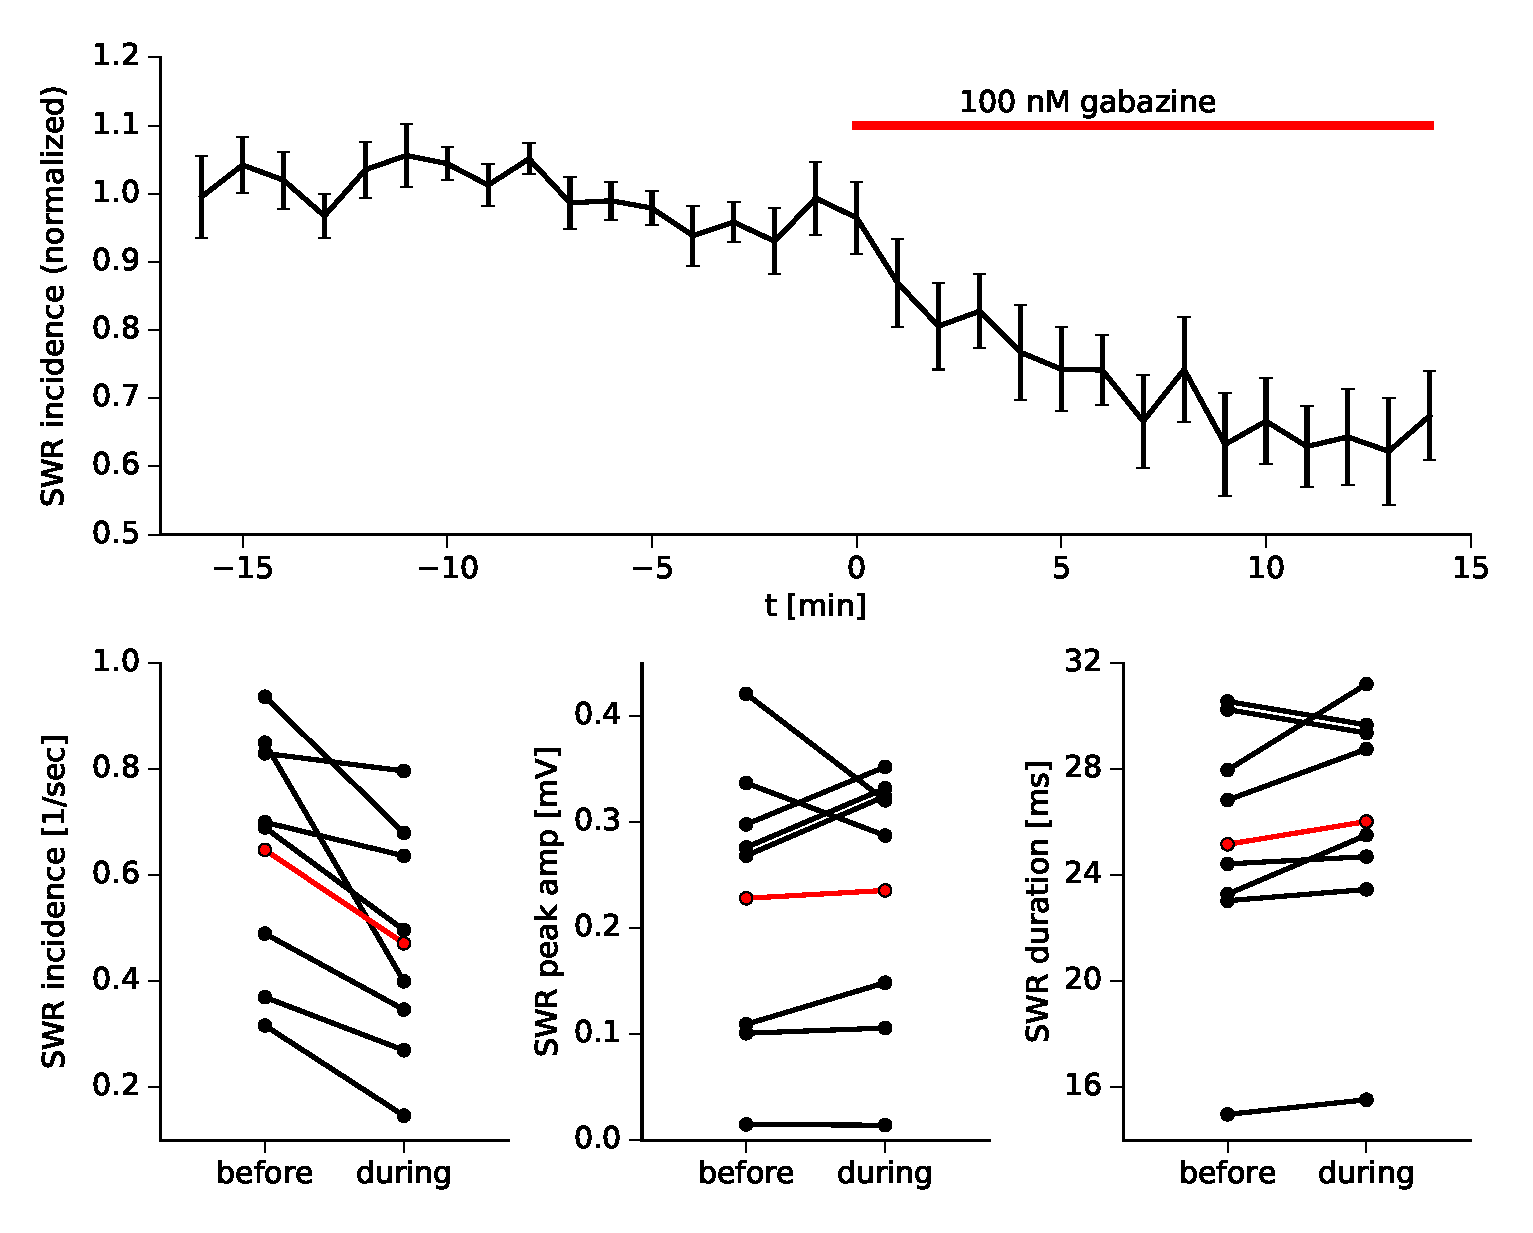
\includegraphics[width =35pc]{gabazine_events_all.eps}
      \caption{
        $\rm GABA_AR$ antagonist gabazine effects on sharp waves. {\bf top}: SW
        incidence in time aggregated from all recordings ($n=8$), where the
        incidence is normalized to 1 by dividing by the mean incidence from before
        the drug application. The red bar shows the time of drug application.
        {\bf bottom:} The average SW incidence, peak and duration measured in
        5-minutes time windows before ([-7, 2] minutes) and during ([6, 11]
        minutes) gabazine application for each slice are denoted with black
        dots. The red dots are the averages from all slices.
      }
      \label{fig:gabazine_sum}
    \end{figure}

    To better characterize how the drug affects the network dynamics, further,
    the analysis focuses on the events in constrained time windows only. Events
    from the window [-7, -2] minutes (before drug application) and [6, 11]
    minutes (after drug application) were used to calculate properties of SWs
    (Figure~\ref{fig:gabazine_sum} bottom row). As already mentioned, there is
    a significant effect on the incidence (around 37\% decrease on average).
    However, somewhat weaker effects are observed on the SW peak amplitude and
    duration.  On average, events tend to get bigger after gabazine
    application. 4 out of 8 recordings show significant (p-value$<0.002$)
    increase in SW amplitude peak after the drug application, and 2/8 show a
    decrease in amplitudes. It is not known whether this increase in amplitudes
    is due to direct effects of gabazine or because of the decreased incidence,
    and thus longer recovery time. 

    The found effect on the SW amplitude is in odds with the finding of
    \citep{Schlingloff2014} who showed that a local puff of gabazine \textit{in
    vitro} decreases the SWR amplitude around the application site
    (Figure~\ref{fig:schlingloff_gabazine}). A possible explanation is that the
    incidence in \citep{Schlingloff2014} is intact as SWRs occur at other
    locations of the slice that are unaffected by the drug. The puffed
    location, however, needs more time to recover from previous events and,
    therefore, the frequent events occurring elsewhere can not engage fully the
    affected subnetwork. In the slices used in our analysis, however, the
    gabazine infusion is global, which results in a slight increase of the SWR
    peaks and also a decrease of the incidence.
    
    \begin{figure}
      \includegraphics[width =35pc]{Schlingloff_3bcd5e.png}
      \caption{A local application of gabazine decreases the amplitude of the
        local SWRs (B) and also decreases the multiunit activity during SW
        events (C, D). Gabazine puffed in the somatic region of PVBCs leads to
        an increased firing and removes the ripple-lock firing of PVBCs. This
        figure is adopted with permission? from \cite{Schlingloff2014}.
      }
    \label{fig:schlingloff_gabazine}
    \end{figure}

    Does gabazine have an effect on the serial correlation between consecutive
    events? To answer this question, the serial correlations (peak-interval and
    interval-peak) were measured before and after drug application in 5-minute
    time windows as described above (Figure~\ref{fig:gabazine_SCsumm}). While
    the peak-interval correlation remains low and does not change after the
    gabazine application, there is a trend of increase in the interval-peak
    correlation. Showing the relation between incidence and interval-peak
    correlation for individual recording (Figure~\ref{fig:gabazine_SCsumm})
    reveals the tendency of decreasing incidence and increased interval-peak
    correlations (6 out of 8 recordings).

    \begin{figure}
      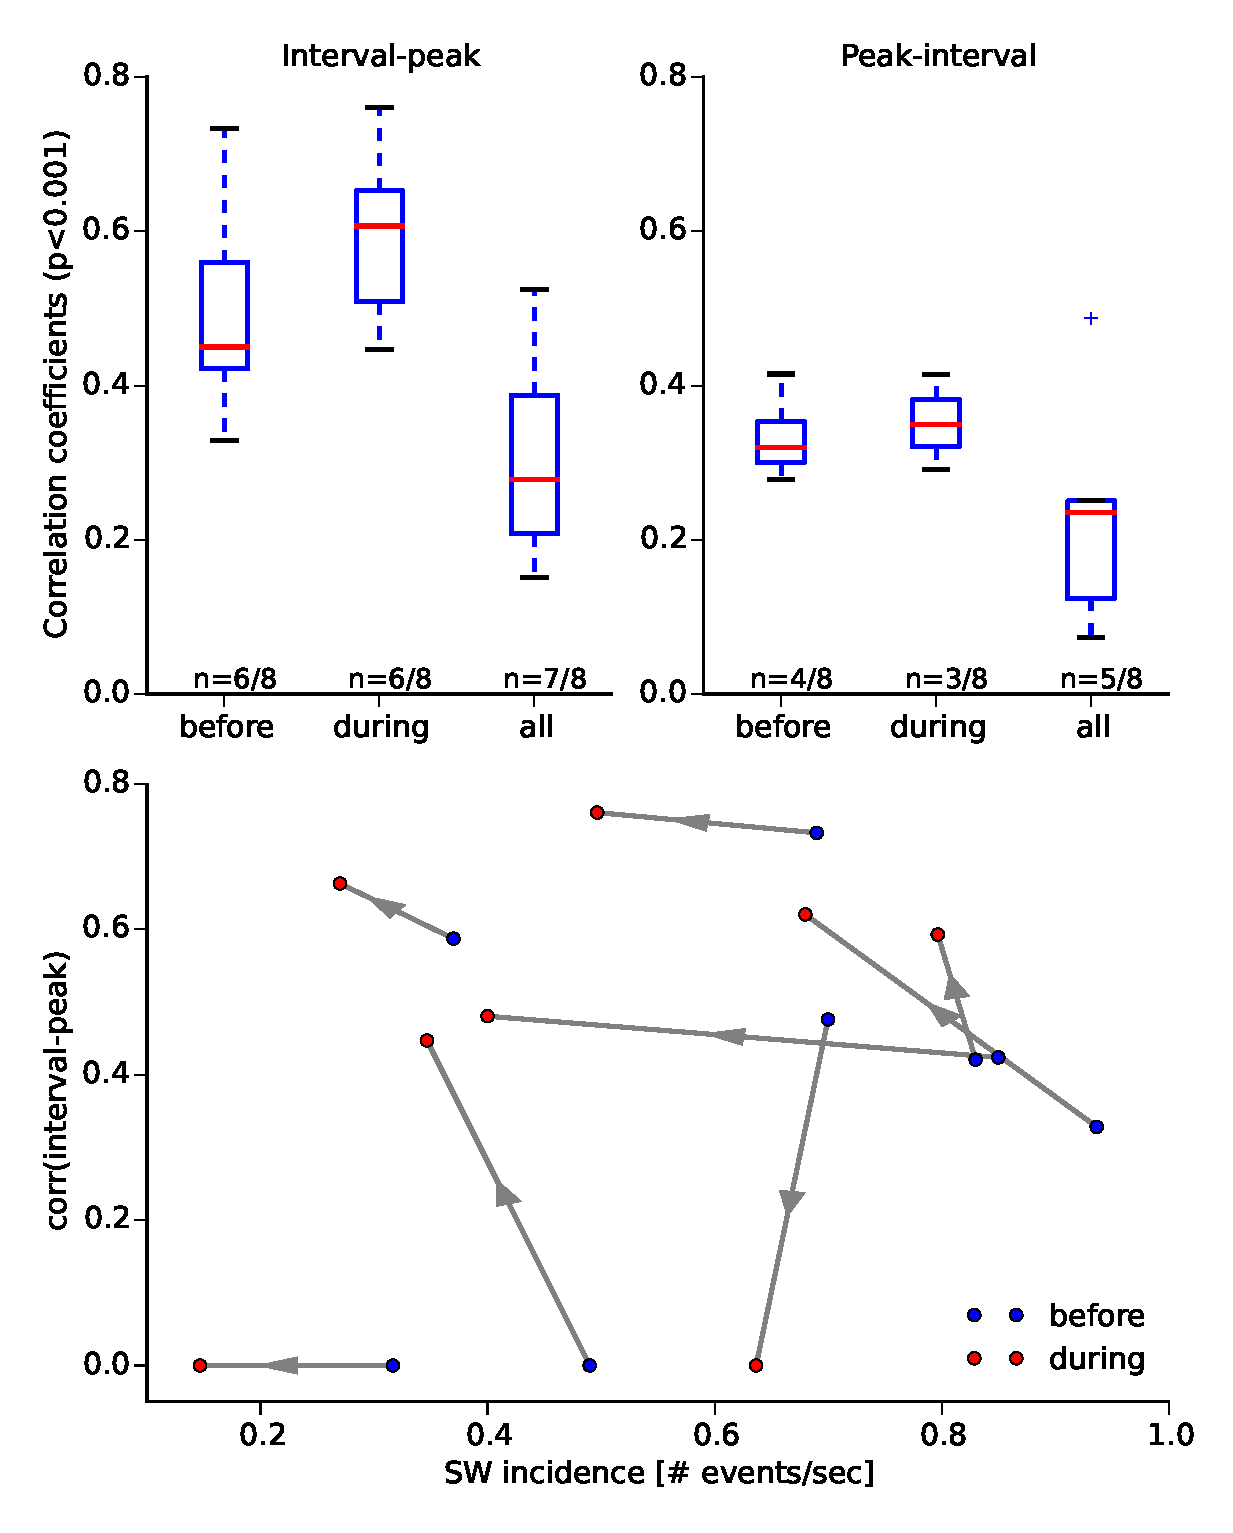
\includegraphics[width= 30pc]{gabazine_SCsumm.eps}
      \caption{
        Gabazine effect on the serial (interval-peak) correlations. \textbf{top:} Serial
        correlation before and during gabazine are calculated in 5-minute long
        time windows, where $n$ shows the number of recordings with significant
        correlations ($p<0.001$) before gabazine application (before), during
        application (during), and aggregated data from the whole recording (all). \textbf{bottom:}
        Serial correlations coefficients between time interval since last event and the following SW
        peak are plotted against recorded incidence; arrows show the change
        after gabazine application.
             }
    \label{fig:gabazine_SCsumm}
    \end{figure}

    In summary, gabazine has the contra-intuitive effect of decreasing the
    incidence of SWRs. Moreover, gabazine application has weak effects in
    increasing the SWR amplitudes and the serial correlations between
    inter-sharp-wave interval and the peak of the following SWR. However, due
    to the small dataset (8 recordings), I can not present a conclusive
    evidence of the drug effects.

  \subsection{Gabazine influence on SWR incidence {\textit {in silico} }}
    \label{sec:gabazine_insilico}
    To better understand how gabazine affects the incidence of SWRs
    {\textit {in silico}}, I deploy the assembly-sequence concept (described in
    Chapter~\ref{chap:memoryreplay}) as a model for the spontaneously occurring
    SWs. Here, numerical simulations of balanced networks with embedded assembly
    sequences and a linear firing rate model are used as tools to describe the
    network dynamics under the influence of gabazine.
      
    In the numerical simulations, sequences of neural assemblies consisting of
    both excitatory and inhibitory neurons are embedded into a randomly
    connected network. Recurrent connectivity ($p_{\rm rc}=0.08$) describes the
    connection probability within an assembly while a feedforward connectivity
    ($p_{\rm ff}=0.06$) is the connectivity between the excitatory neurons of
    consequent assemblies in the sequence (sketch of network connectivity is
    shown in Figure~\ref{fig:net_sketch}). With these parameters values, noise
    fluctuations in the firing rates get amplified by the feedforward structure
    resulting in spontaneous replays (Figure~\ref{fig:spontan}). For a more
    detailed description of the numerical model and the parameter values,
    please refer to Chapter~\ref{chap:memoryreplay}. Here, the effects of
    gabazine are modeled simply by decreasing the conductances of the targeted
    inhibitory synapses with a fixed rate (i.e., $5\%$).

    Not surprisingly, gabazine drastically increased the rate of spontaneous
    replays of assembly sequences in the modelled network. This is illustrated
    in Figure~\ref{fig:gabzine_sim}, where gabazine is applied to all inhibitory
    synapses after the $21^{\rm st}$~second of the simulation. The top two
    panel show raster plots of the excitatory and inhibitory neurons where the
    black dots show individual spikes, and the black stripes are burst of
    synchronous activity during which many neurons fire in close temporal
    proximity. The replays during these activity bursts are used as a model of
    the sharp-wave events. The frequency of these population events is
    increased immediately after the simulated gabazine infusion, as seen in the number of
    replays (the top panel), and in the firing rates (third panel). This result
    is in direct opposition with the gabazine effects that are reported
    {\textit{in vitro}} (Section~\ref{gabazine_invitro}).

    \begin{figure}
      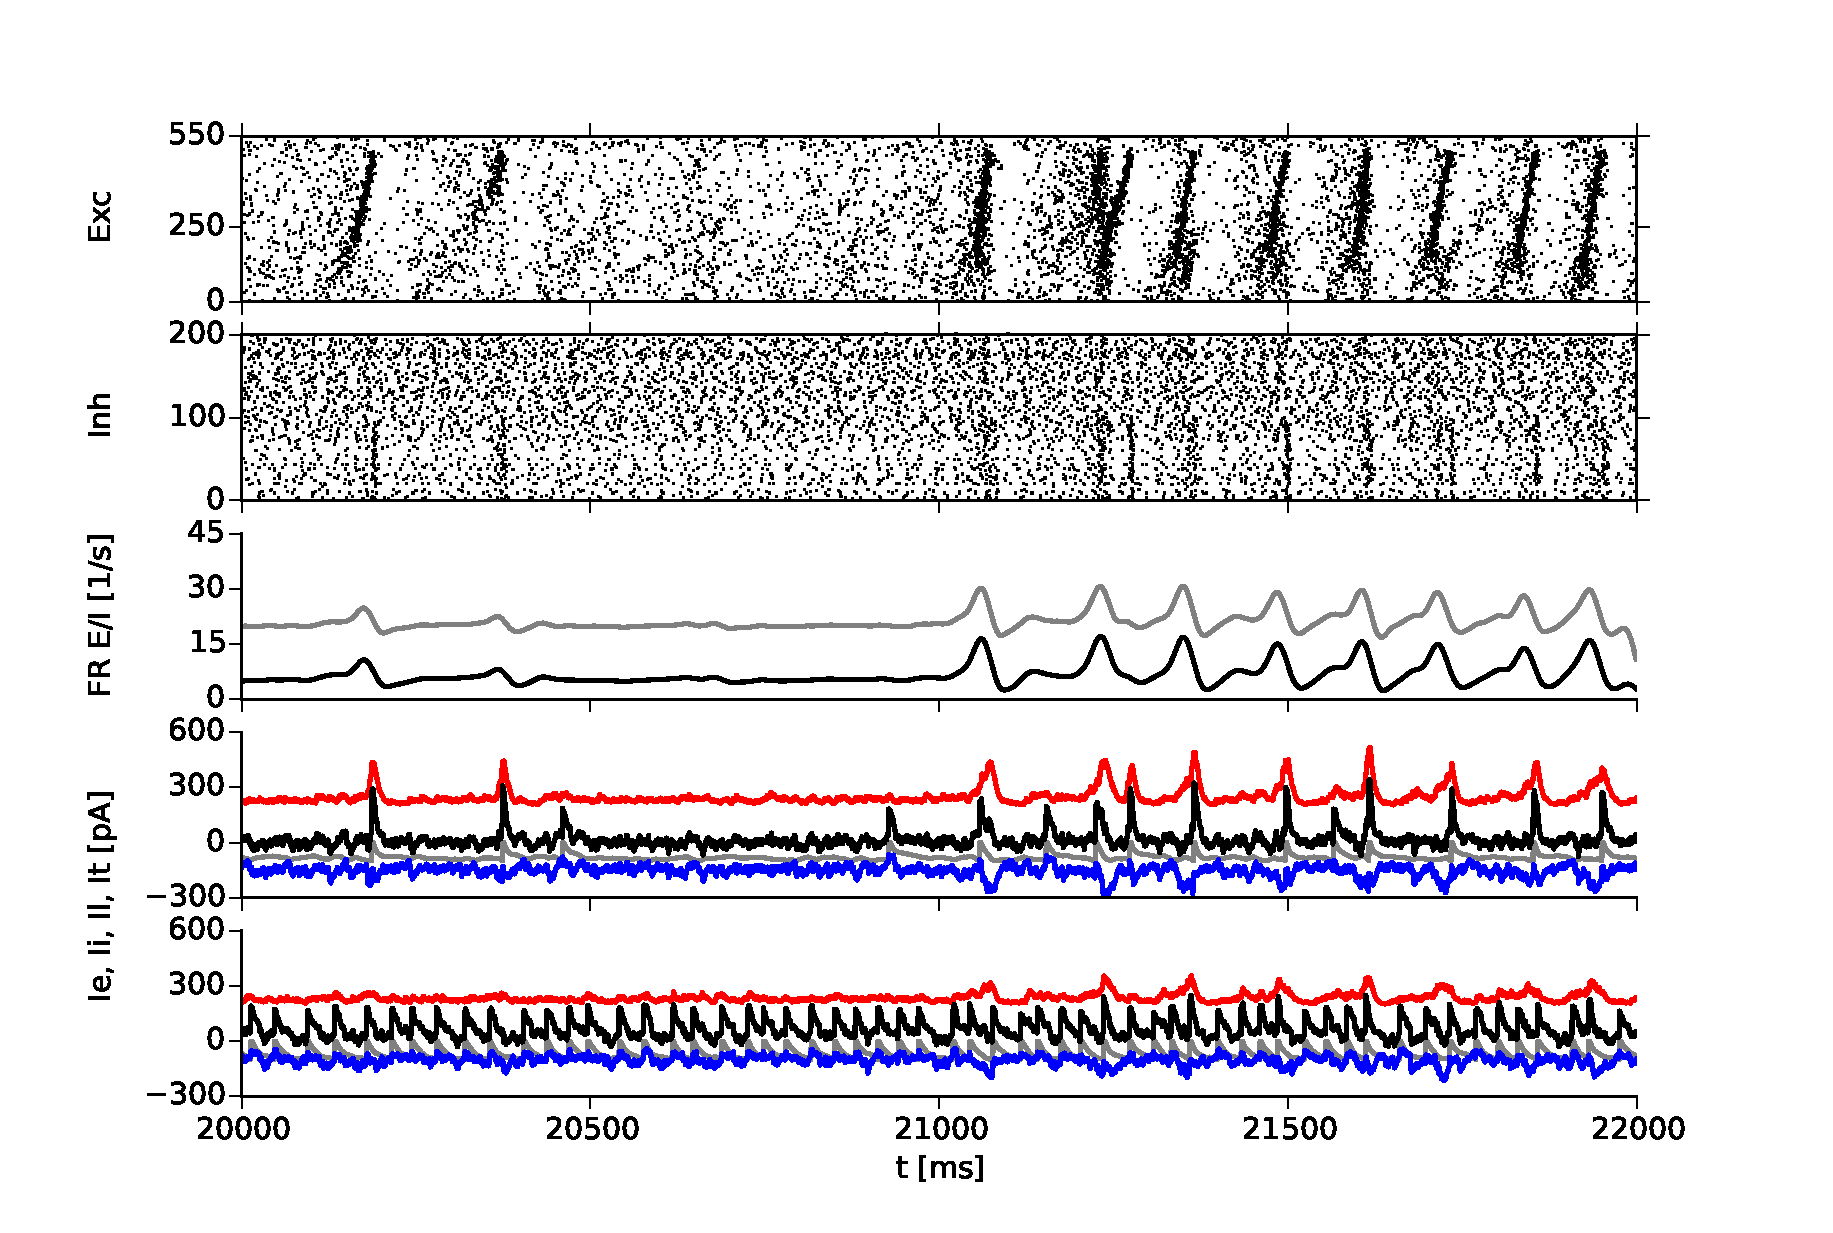
\includegraphics[width =35pc]{gabazine_sim.eps}
      \caption{
        Gabazine {\it in silico} increases the rate of spontaneous replays.
        Decreasing all inhibitory conductances (at $21^{\rm th} \rm second$
        with 5\% leads to increase in the incidence of spontaneous replays in
        balanced-network simulations. The two upper panels show rater plots of
        subpopulations of excitatory and inhibitory neurons, where each black
        dot denotes a spike. Middle plot shows the firing rate of the
        excitatory and inhibitory populations. The last two panels show the
        currents experienced by one excitatory and one inhibitory neuron. Red,
        blue, gray, and black color denote excitatory, inhibitory, leak, and
        total currents.
            }
    \label{fig:gabazine_sim}
    \end{figure}

    Can a relatively simple two-populations balanced network explain the
    gabazine-associated decrease of SWR incidence reported in experiments?
    $\rm GABA_A$ receptors ($\rm GABA_A R$) are known to be complex channels
    with six subunits that can come in various combinations (for the curious
    readers, see Section~\ref{sec:gabaa_intro}). The expressed subunits largely
    determine the receptor properties, i.e., time constants, affinity to GABA
    and other neurotransmitters. For example tonic $\rm GABA_A R$ are
    insensitive for gabazine at low concentrations while phasic $\rm GABA_A R$
    show various affinities depending on the subunit expression. The subunit
    expression is largely determined by the type of the postsynaptic neuron and
    by the location of the channels on the morphological tree
    \ref{???}. One hypothesis to explain the gabazine-associated decrease of SW
    events relies on the assumption that gabazine has differential effects on
    the different $\rm GABA_A$ synapses. And more specifically, if
    inhibitory-to-inhibitory synapses are affected to a larger degree than the
    inhibitory-to-excitatory synapses, one would expect a network that is less
    disinhibited, and thus, the excitatory population receives more inhibition
    resulting in smaller firing rates. In what follows, I test whether such
    assumptions would really decrease the incidence of modeled events.

    As a toy example in numerical simulation, I consider the extreme case where
    gabazine affects the inhibitory-to-inhibitory synapses only. As expected,
    the firing rate of the excitatory neurons is decreased
    (Figure~\ref{fig:gabazine_sim_giionly}). However, the network shows a
    decrease in the firing rate of the inhibitory population as well. How is it
    possible that excitatory neurons receiving weaker inhibition (smaller input
    rate), fire less? To better understand the effects of gabazine, further, I
    present an analytical approach.
    
    \begin{figure}
      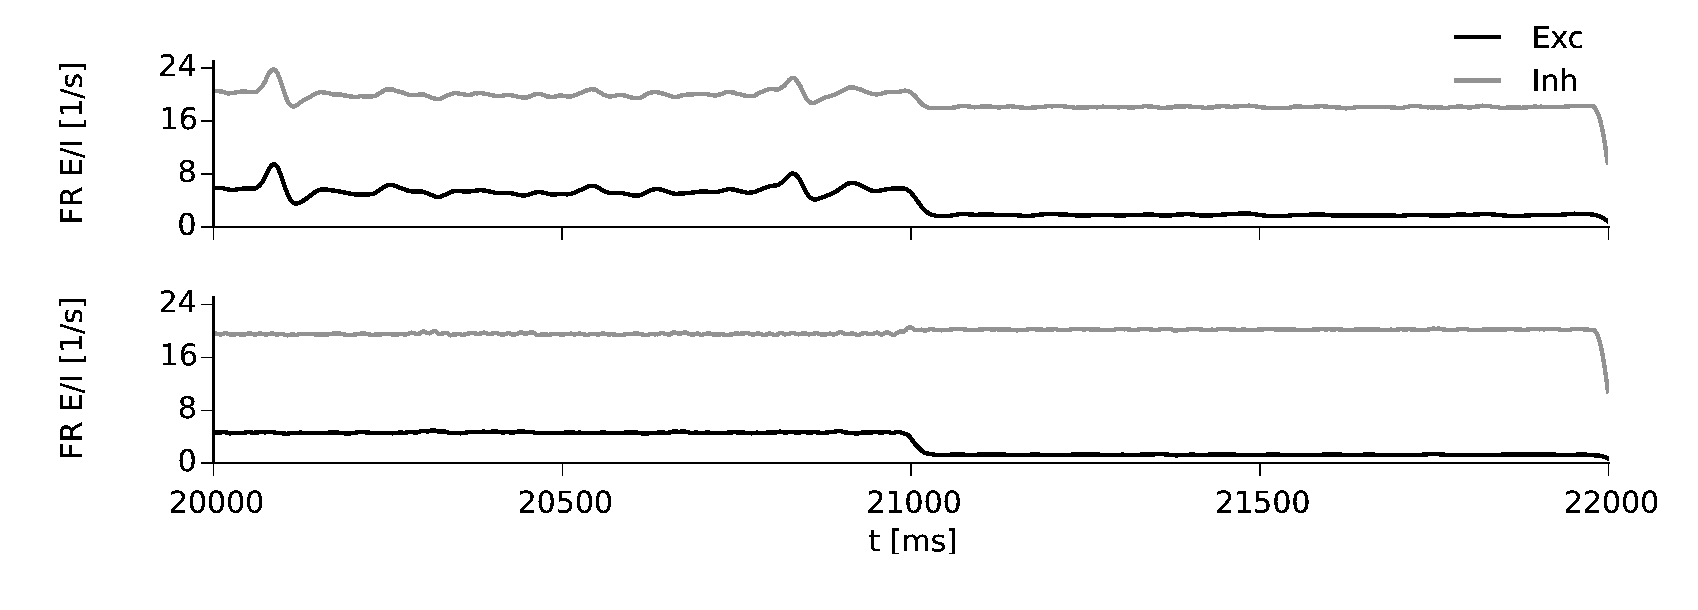
\includegraphics[width =35pc]{gabazine_sim_gii.eps}
      \caption{
        Gabazine {\it in silico} applied only to inhibitory-to-inhibitory synapses
        decreases the rate of spontaneous replays. {\bf top:} Spontaneous replays
        occur during the peaks of the excitatory and inhibitory firing rates. 
        Decreasing the inhibitory-to-inhibitory conductances (at $21^{\rm th} \rm second$
        with 5\% decreases of firing rates and abolishes the spontaneous replays in
        balanced-network simulations. {\bf bottom:} Figure-out what I did! small gee?
      }
    \label{fig:gabazine_sim_giionly}
    \end{figure}

    To capture the network dynamics, I apply a linear model of a two-population
    balanced network and analyse how the rates depend on gabazine. The network
    dynamics is described by the system of differential equations:
    \begin{equation}
      \begin{split}
        \tau \frac{\text{d}r^E}{\text{d}t} &= - r^E + w_{\rm ee} \, r^E -w_{\rm ei} \, r^I + I_0\\
        \tau \frac{\text{d}r^I}{\text{d}t} &= - r^I + w_{\rm ie} \, r^E -w_{\rm ii} \, r^I + I_0\\
      \end{split}
      \label{eq:balanced_net}
    \end{equation}
    where $r^E$ and $r^I$ are excitatory and the inhibitory firing rates,
    respectively. The connection from population $x$ to $y$ is described by the
    connection weight $w_{\rm yx}$ ($x,y = e, i$). The population time constant
    is $\tau$, and the external input to the populations is denoted with $I_0$.

    Assuming that the network is in a steady state, then the rates are
    constant, i.e., $ \frac{\text{d}r^E}{\text{d}t} = 0$ and
    $\frac{\text{d}r^I}{\text{d}t} = 0 $. In this condition, one can express
    the stationary solution:
    \begin{equation}
      \begin{split}
        r^E &= \frac{(1+w_{\rm ii} - w_{\rm ei})}{w_{\rm ie}w_{\rm ei} -
                (1+w_{\rm ii})(-1+w_{\rm ee})} I_0 \\
        r^I &= \frac{(1+w_{\rm ie} - w_{\rm ee})}{w_{\rm ie}w_{\rm ei} -
                (1+w_{\rm ii})(-1+w_{\rm ee})} I_0
      \end{split}
      \label{eq:balanced_sol}
    \end{equation}
  
    To estimate how gabazine-induced decrease of inhibitory connections
    affects the firing rates, we can look at the derivatives of the
    steady-state rates in respect to the gabazine concentration $c_{\rm gbz}$:
    \begin{equation}
      \frac{\partial r^E}{\partial c_{\rm gbz}} =
      \frac{\partial r^E}{\partial w_{\rm ei}} \cdot \frac{\partial w_{\rm ei}}{\partial c_{\rm gbz}} + 
      \frac{\partial r^E}{\partial w_{\rm ii}} \cdot \frac{\partial w_{\rm ii}}{\partial c_{\rm gbz}}
      \label{eq:re_chain}
    \end{equation}
    and
    \begin{equation}
      \frac{\partial r^I}{\partial c_{\rm gbz}} =
      \frac{\partial r^I}{\partial w_{\rm ei}} \cdot \frac{\partial w_{\rm ei}}{\partial c_{\rm gbz}} + 
      \frac{\partial r^I}{\partial w_{\rm ii}} \cdot \frac{\partial w_{\rm ii}}{\partial c_{\rm gbz}}.
      \label{eq:ri_chain}
    \end{equation}

    The partial derivatives of inhibitory weights ($w_{\rm ei}$ and $w_{\rm
    ii}$) in respect to the drug concentration $c_{\rm gbz}$ is negative due to
    the antagonist  effects of gabazine. The partial derivatives of the rates
    in respect to the inhibitory weights can easily be estimated from
    Equation~\ref{eq:balanced_sol}:
    \begin{equation}
      \begin{split}
        \frac{\partial r^E}{\partial w_{\rm ii}} &= 
              I_0 \frac{w_{\rm ei} (1 + w_{\rm ie} - w_{\rm ee})} {D^2} \\
        \frac{\partial r^I}{\partial w_{\rm ii}} &=
              I_0 \frac{(-1 + w_{\rm ee})(1 + w_{\rm ie} - w_{\rm ee})} {D^2} \\
      \end{split}
      \label{eq:drdwii}
    \end{equation}

    \begin{equation}
      \begin{split}
        \frac{\partial r^E}{\partial w_{\rm ei}} &=
              I_0 \frac{-(1 + w_{\rm ii}) (1 + w_{\rm ie} - w_{\rm ee})} {D^2} \\
        \frac{\partial r^I}{\partial w_{\rm ei}} &=
              I_0 \frac{-w_{\rm ie} (1 + w_{\rm ie} - w_{\rm ee})} {D^2} \\
      \end{split}
      \label{eq:drdwei}
    \end{equation}
    where $D=w_{\rm ie}w_{\rm ei} - (1+w_{\rm ii})(-1+w_{\rm ee})$.
    
    If we now assume that gabazine has the same effect on all inhibitory
    synapses, i.e., $\frac{\partial w_{\rm ei}}{\partial c_{\rm gbz}} =
    \frac{\partial w_{\rm ii}}{\partial c_{\rm gbz}}$, the change of firing
    rate due to gabazine is:
    \begin{equation}
      \begin{split}
        \frac{\partial r^E}{\partial c_{\rm gbz}} &=
            \frac{\partial w_{\rm ii}}{\partial c_{\rm gbz}} \cdot
            I_0 \frac{-(1 + w_{\rm ii} - w_{\rm ei}) (1 + w_{\rm ie} - w_{\rm ee})} {D^2} =
            - \frac{\partial w_{\rm ii}}{\partial c_{\rm gbz}} \cdot \frac{r^E r^I}{I_0} > 0 \\
        \frac{\partial r^I}{\partial c_{\rm gbz}} &=
            \frac{\partial w_{\rm ii}}{\partial c_{\rm gbz}} \cdot
            I_0 \frac{- (1 + w_{\rm ie} - w_{\rm ee})^2} {D^2} =
            - \frac{\partial w_{\rm ii}}{\partial c_{\rm gbz}} \cdot \frac{r^I r^I}{I_0} > 0 \\
      \end{split}
      %\label{eq:x}
    \end{equation}
    In line with the simulations, the derivatives above are always positive (if
    $\frac{\partial w_{\rm ii}}{\partial c_{\rm gbz}} < 0 $), i.e., gabazine
    always increases the rate of both excitatory and inhibitory
    populations. 

    Can this linear model model explain the simulation results in which
    gabazine affects only inhibitory-to-inhibitory synapses? There we saw a
    decrease not only in the excitatory but also in the inhibitory firing rates
    (Figure~\ref{fig???,bottom?}). Taking the rate derivatives in respect to
    $w_{\rm ii}$ only (In Equations~\ref{eq:re_chain} and \ref{eq:ri_chain}, we
    assume that $\frac{\partial w_{\rm ei}}{\partial c_{\rm gbz}} = 0$):

    \begin{equation}
      \begin{split}
        \frac{\partial r^E}{\partial c_{\rm gbz}} &=
            \frac{\partial w_{\rm ii}}{\partial c_{\rm gbz}} \cdot
            I_0 \frac{w_{\rm ei}(1 + w_{\rm ie} - w_{\rm ee})} {D^2} =
            \frac{\partial w_{\rm ii}}{\partial c_{\rm gbz}} \cdot \frac{w_{\rm ei}}{D} \cdot r^I \\
        \frac{\partial r^I}{\partial c_{\rm gbz}} &=
            \frac{\partial w_{\rm ii}}{\partial c_{\rm gbz}} \cdot
            I_0 \frac{(-1+w_{\rm ee}) (1 + w_{\rm ie} - w_{\rm ee})} {D^2} =
            \frac{\partial w_{\rm ii}}{\partial c_{\rm gbz}} \cdot \frac{-1+w_{\rm ee}}{D} \cdot r^I \,\, . \\
      \end{split}
      %\label{eq:x}
    \end{equation}
 
    Here, the sign of the determinant $D$ from Equation~\ref{eq:balanced_net}
    determines the change in firing rate. Let us first assume that $D<0$. To
    fulfil the requirement for positive firing rates (i.e., $r^I>0$ in
    Equation~\ref{eq:balanced_sol}), then $w_{\rm ee}>1+w_{\rm ie}$ should be
    fulfilled. However, this is unlikely to be the case as the excitatory
    conductances used in the simulations are all equal $g_{\rm ee}=g_{\rm ie}$.
    Therefore, I conclude that $D>0$. In that case, it is easy to see that
    $\frac{\partial r^E}{\partial c_{\rm gbz}} < 0$, meaning that excitatory
    rate decreases when $w_{\rm ii}$ is depressed. This line of arguments is
    supported by the simulations, where gabazine applied to the
    inhibitory-to-inhibitory connections only decreases the excitatory firing
    rate (Figure~\ref{fig:gabazine_sim_giionly}). On the other hand, $r^I$
    shows more interesting behaviour that depends on the excitatory weights.
    For intermediate values $w_{\rm ee} \in (1, 1+w_{\rm ie})$, the inhibitory
    rate decreases during gabazine application as well (as seen in
    Figure~\ref{fig:gabazine_sim_giionly}, top panel). For values of $w_{\rm
    ee}$ outside of this interval, one would expect increase of inhibitory
    firing after the drug infusion. For the prove of concept, I tested a
    network where $g_{\rm ee}=2 g_{\rm ie}$ and show that in such case the
    inhibitory rate goes up after the simulated drug application
    (Figure~\ref{fig:gabazine_sim_giionly}, bottom panel).
    %To test again whether low/high wee increases ri!!!!
    %I tested that by using lower (5 times smaller than default)
    %and higher (5 times larger than default) excitatory-to-excitatory
    %connectivity in the numerical model and found that inhibitory rate is
    %indeed increased (not shown here).

    To summarize the results from this section, by using numerical simulations
    and a linear analytical description, I showed that in a balanced network a
    gabazine application is increasing the firing rates of both inhibitory and
    excitatory populations. This increase of firing leads to higher incidence
    of spontaneous replays which is in odds with the counterintuitive decrease
    of incidence observed {\textit {in vitro}}. Therefore, I tested whether a
    differential effect of gabazine on different synapses can explain the
    experimental results. I considered the extreme case when gabazine affects
    only inhibitory-to-inhibitory synapses and showed that in this case we can
    always expect decrease in the rate of excitatory population. This result
    suggests that possibly stronger effects of gabazine on the inhibitory
    neurons might explain the decreased SWR incidence after gabazine
    application {\textit {in vitro}}.
    
    Here I examine a minimal model consisting of only two populations, but
    nevertheless the approach can provide some means for studying {\it in-vitro}
    models. A similar approach can also be applied to the more accurate
    3-population nonlinear model currently developed by Roberta Evangelista,
    and utilized to examine in what conditions gabazine decreases the network
    excitability. Is it possible that in the 3-population model, a gabazine
    application to all inhibitory synapses can decrease the rate of spontaneous
    events? Or would it be required that the disinhibitory synapses (from PVBC
    to the mysterious inhibitory neurons) are affected to a larger degree?

    A strong assumption in the foundation of the current framework is that the
    decrease of SWR incidence is due to decrease of firing of the excitatory
    population. Whether this is indeed the case has to be confirmed from
    {\it in-vitro} experiments. It is also not known how does gabazine affects the
    firing of the inhibitory populations. The simulations show that gabazine
    applied only on the inhibitory-to-inhibitory connections can decrease not
    only the excitatory but also the inhibitory firing rates. This result is
    interesting by its own as the decrease of $r^E$ is counterintuitive. How
    does it come that the excitatory population decreases its firing rate after
    receiving less inhibition due to the decrease of $r^I$? (should I dive into that??)

  \subsection{Involvement of $\rm GABA_B$ receptors in sharp waves}

    Sharp waves are huge population events where many pyramidal cells and
    interneurons are firing with increased firing rates, which is especially
    pronounced for the perisomatic targeting parvalbumin-positive basket cells
    (PVBCs) and the bistratified cells \citep{Klausberger2009}. It has been
    shown that the repetitive firing of interneurons can activate extrasynaptic
    $\rm GABA_B$ receptors possibly through increased concentrations of ambient
    GABA in the extracellular space \cite{Wang2010,??}. The inhibition from
    $\rm GABA_B Rs$ is relatively slow, lasting several hundreds of
    milliseconds, which is close to the time scale of the typical inter-SW
    intervals. Here, I study the possibility that the relatively long time
    intervals between SW events are determined by $\rm GABA_B Rs$.
    
    First, to investigate whether $\rm GABA_B$ is involved in the SW incidence
    in the {\textit{in-vitro}} model, I analysed extracellular recordings where
    the $\rm GABA_B R$ antagonist SCH50,911 (further referred as SCH) was
    applied in slices. The number of analysed slices is 12 (see the Methods
    section). An example of the SCH effects in a slice are shown in
    Figure~\ref{fig:gB_example}. The drug effects are reflected in the network
    dynamics already during the first minute of application by increasing the
    incidence of SWs (Figure~\ref{fig:gB_example}, top panel). An independent
    two-sample t-test of the incidence (measured as number of events per sweep
    in confined 5-minute time intervals) show a significant increase of
    incidence (p-value $<10^{-7}$). Other main properties, such as, peak
    amplitude and duration are decreased after the SCH application (p-values
    $<10^{-10}$, and $<10^{-3}$, respectively).
    
    \begin{figure}
      %\includegraphics[width =35pc]{19march13_slice1.png}
      \includegraphics[width =35pc]{20jan12_slice2.png}
      \caption{ 
        Extracellular recording from the CA3 area where SCH50,911 is applied to
        the hippocampal slice. The time of drug application is denoted with a
        horizontal red bar. The top panel shows the SW incidence in time with a
        minute time resolution. The two panels below show the SW amplitude
        peaks, where `fil' and `raw' stand for band-passed filtered ($\sim
        5-50\, \rm Hz$, for details see the Methods section) and raw voltage
        traces, respectively; units are in mV. The gray dots represent single
        events, and the black lines represent the mean and the standard
        deviation of the amplitude peak in a minute time window. Analogously,
        the forth panel shows the SW duration in milliseconds. The panels on
        the bottom row show all events before (left) and during (middle) drug
        application overlaid in gray, and the mean wave-forms are in black. The
        right-most panel shows a comparison between the mean events from before
        and during SCH application.
              }
    \label{fig:gB_example}
    \end{figure}

    Blocking the $\rm GABA_B Rs$ resulted in increase of the average incidence
    of spontaneous sharp waves from all slices.  The drug effects are visible
    already in the first minute after the application and saturate around 2-3
    minutes later (Figure~\ref{gB_summ}, top panel). To better assess the
    effects of SCH further, the analysis focuses on the events in 5-minutes
    long time windows, i.e., in the intervals [-5, 0] that is before and [2, 7]
    minutes that is during drug application. Comparing the data from these two
    intervals shows that SCH increases the incidence in every recording, and
    10/12 show a significant increase (independent 2-sample t-test;
    p-value$<0.002$). On average, SCH resulted in decrease of SW amplitudes
    (Figure~\ref{gB_summ}, bottom middle panel), where 6/12 slices show
    a significant decrease (p-value$<0.001$), and in 2/12 slices the amplitudes
    were increased (p-value$0.001$). The duration of sharp waves, also
    decreases on average, but however, this change is not significant
    (p-value$>0.01$ in 11/12 slices). While the result for every recording
    varies depending on the exact 5-minute time windows that are used for the
    analysis, the summary results do not change qualitatively.
    
    \begin{figure}
      \includegraphics[width =35pc]{SCH_all.eps}
      \caption{
        $\rm GABA_BR$ antagonist SCH50,911 effects on sharp waves. {\bf top}:
        SW incidence in time aggregated from all recordings ($n=12$), where the
        incidence is normalized to 1 by dividing by the mean incidence before
        the drug application. The red bar shows the time of drug application.
        {\bf bottom:} The average SW incidence, peak and duration measured in
        5-minutes time windows before ([-5, 0] minutes) and during ([2, 7]
        minutes) SCH application for each slice are denoted with black dots.
        The red dots are the averages from all slices.
            }
    \label{gB_summ}
    \end{figure}

    Next, I inquire whether blocking $\rm GABA_B Rs$ affects also the serial
    correlation between events. At first glance the pooled data does not reveal
    any change in the correlations, as the correlation distributions from
    before and during SCH application (Figure~\ref{gB_SCsumm}, top panels) are
    statistically similar. However, looking at the effects in the individual
    recordings (Figure~\ref{gB_SCsumm}, bottom panel) one can see that there is
    a decrease of serial correlation after drug application in 10 out of 12
    slices (the 2 remaining recordings show no significant correlations).

    \begin{figure}
      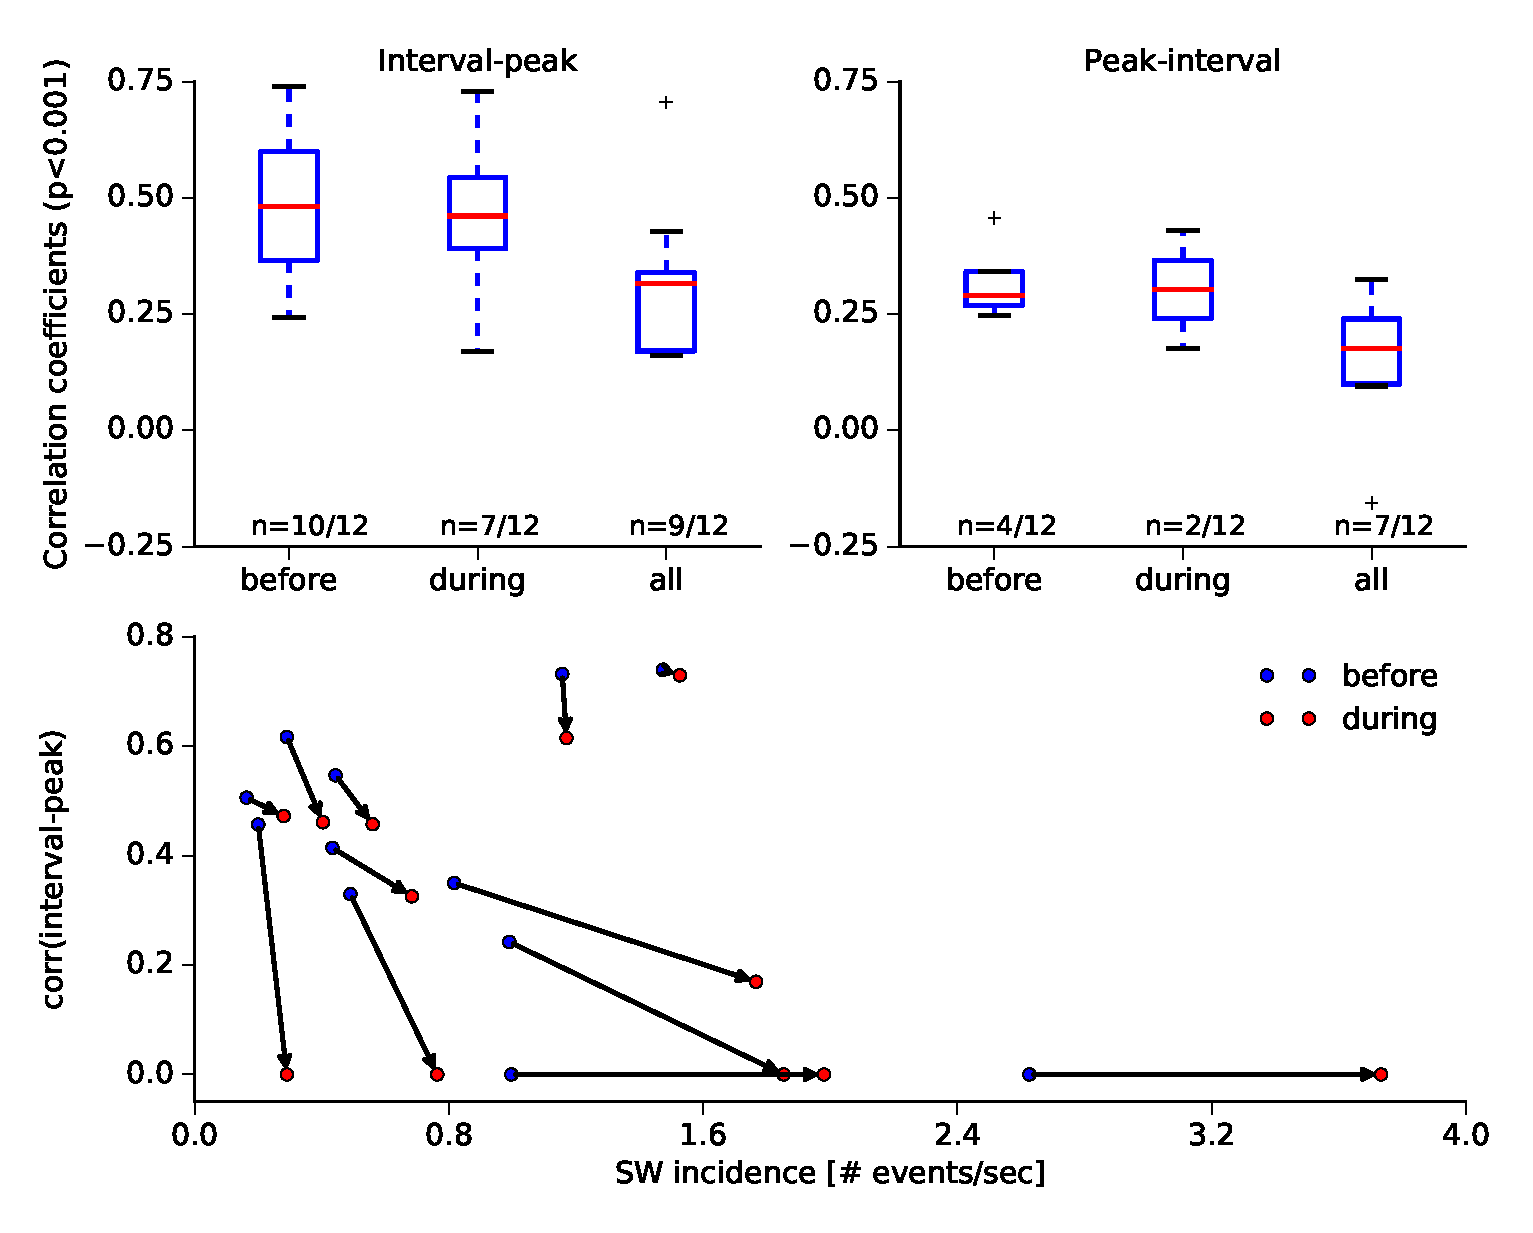
\includegraphics[width =35pc]{SCH_SCsumm.eps}
      \caption{
        $\rm GABA_BR$ antagonist SCH50,911 effect on the serial (interval-peak)
        correlations. \textbf{top:} Serial correlation before and during
        gabazine are calculated in 5-minute long time windows, where $n$ shows
        the number of recordings with significant correlations ($p<0.001$)
        before SCH application (before), during application (during), and
        aggregated data from the whole recording (all). \textbf{bottom:} Serial
        correlations coefficients between time interval since last event and
        the following SW peak are plotted against recorded incidence; arrows
        show the change after SCH application.
            }
    \label{gB_SCsumm}
    \end{figure}

    To summarize the findings above, $\rm GABA_B Rs$ are taking part in the SW
    modulation by increasing the incidence and decreasing the peaks of SWs.
    However, the increase in incidence is on average less than two-fold
    suggesting that there are other mechanisms different than $\rm GABA_B$ that
    act on a slow time scales and are involved in controlling the incidence.
    Moreover, blocking $\rm GABA_B Rs$ leads to a decrease in the serial
    correlations between interval and peaks, which is puzzling given the
    increased incidence. Intuitively, one could expect that the serial
    correlations are stronger for higher incidences, and weaker for lower
    incidences when the system depletion is recovered. To investigate how does
    $\rm GABA_B Rs$ influence the SW incidence, it is worth having a closer
    look at the possible involvement of the different $\rm GABA_B$ channels.

    It is been shown that a repetitive firing of certain interneurons can evoke
    slow and strong inhibition due to activation of postsynaptic or
    extrasynaptic $\rm GABA_B$ receptors on pyramids \citep{Scanziani2000,
    Gassmann2012}. As sharp waves are population events that recruit many
    neurons, and especially the perisomatic targeting interneurons
    \citep{Klausberg2009} it is likely that ambient GABA in this region is
    increased \citep{Hollnagel2014, Lang2014}. Next, I ask whether $\rm
    GABA_BRs$ located postsynaptically on pyramidal cells are indeed activated
    after SWs, and whether they play any role in the modulation of SWs. To test
    this hypothesis, here I analyse data from simultaneous (paired)
    extracellular and intracellular recordings performed in the radiatum layer
    of the hippocampal CA3 area and a pyramidal cell in the CA3, respectively.
    By averaging the intracellular traces across events, we can see that a GB
    hyperpolarization is present in a few recordings, but is not is not visible
    in the mean of all recordings (Figure~\ref{fig:intra_means}, top panel).
    Most intracellular traces show various combination of depolarization and
    hyperpolarization, indicating a rich dynamics of excitatory and inhibitory
    inputs. In the recordings that show a slow hyperpolarization (4 out of 13
    recordings, shown in Figure~\ref{fig:intra_means}, bottom panel) the trough
    in the membrane potential is around $200 \, \rm ms$ after the population
    event and lasts for about $500 \, \rm ms$. Interestingly, only one
    recording reveals well-pronounced slow as well as fast inhibition (red
    trace).

   \begin{figure}
      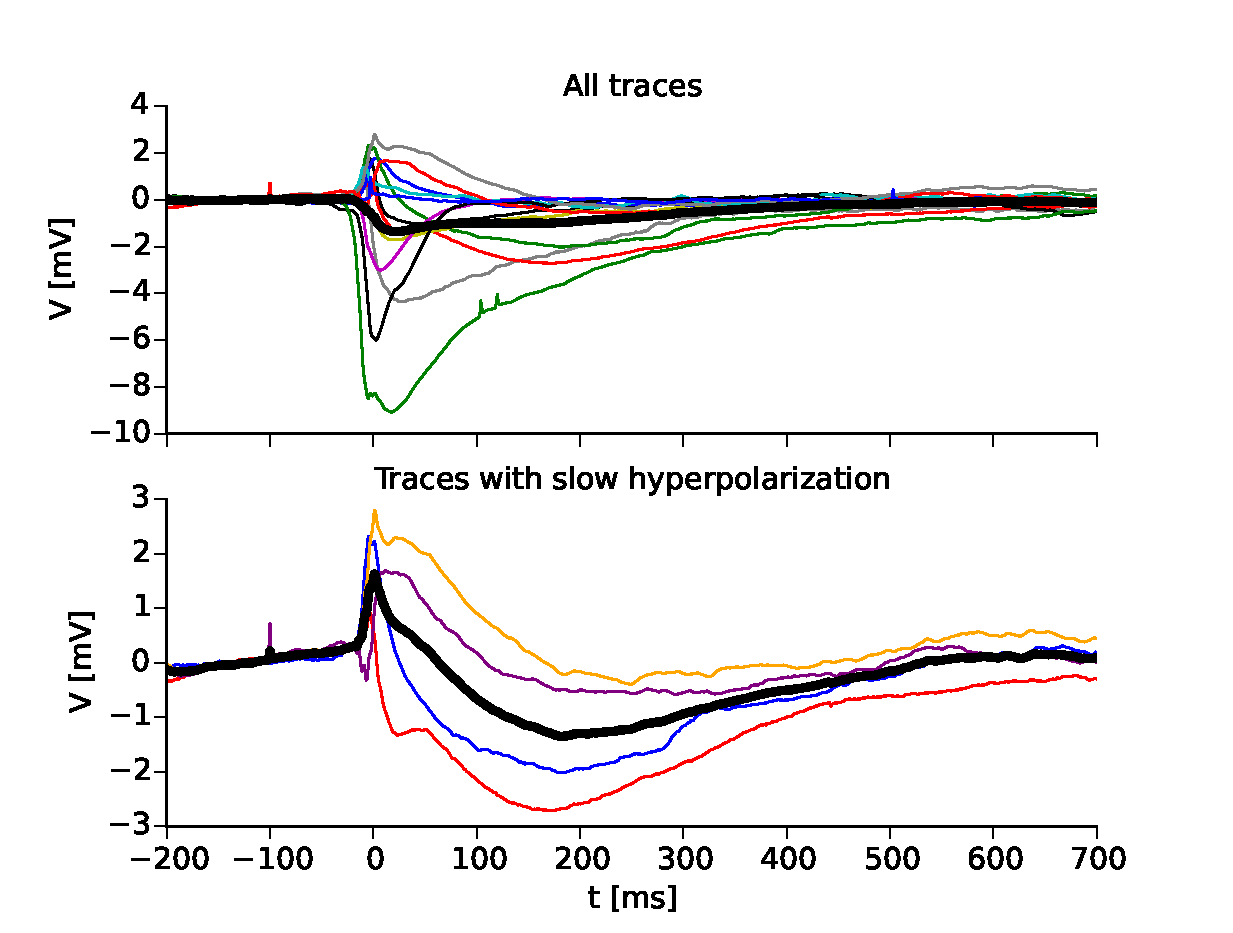
\includegraphics[width =30pc]{mean_intras.eps}
      \caption{ 
        Simultaneous extracellular and intracellular recordings in slices. {\bf
        top:} Intracellular recordings from patched pyramidal cells during
        sharp waves. The mean voltage traces associated to SWs from each slice
        are color coded; the thick black line is the mean of the means. {\bf
        bottom:} Mean voltage traces of cells that show slow, possibly $\rm
        GABA_BR$-evoked hyperpolarization. All traces are normalized by
        subtracting the mean potential the before the event.
              }
      \label{fig:intra_means}
    \end{figure}

    Is the slow hyperpolarization correlated in any way with the amplitude of
    the SWs? To test this, I separated the events in each recording in two
    groups: big and small events, i.e., the 30\% biggest or 30\%
    smallest events, respectively. Plotting the mean intracellular trace during
    small and big events, shows that the SWs with larger amplitudes are
    associated with larger hyperpolarization (Figure~\ref{fig:intra_big_small},
    top panel). Interestingly, the mean traces before big and small events are
    virtually indistinguishable (Figure~\ref{fig:intra_big_small}, bottom
    panel), suggesting that the hyperpolarization does not determine the size
    of the following event. This result holds for all the four recordings that
    exhibit slow inhibition in the voltage potential.
    
    \begin{figure}
      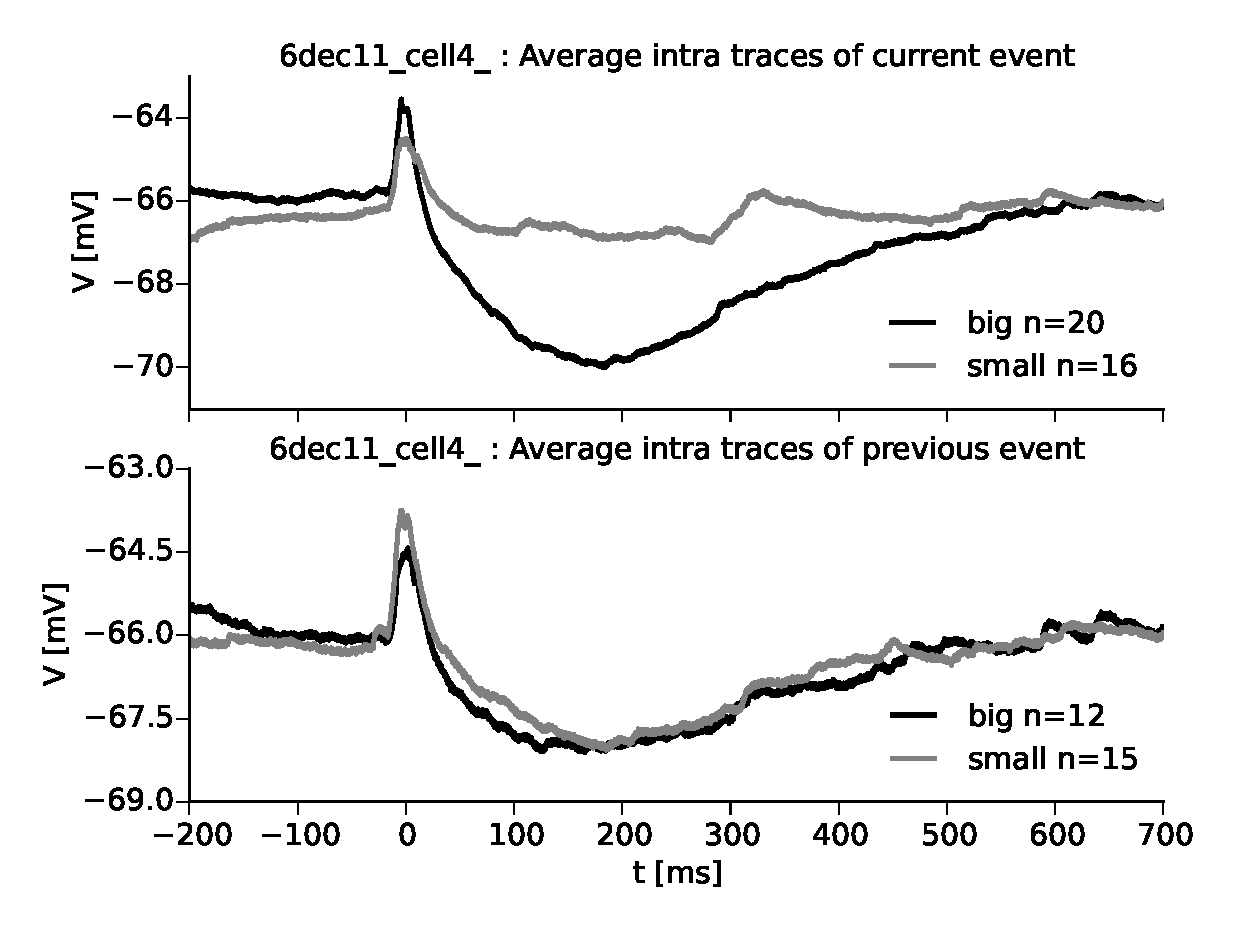
\includegraphics[width =30pc]{6dec11_cell4_000.eps}
      \caption{ 
        Sharp waves with larger peak amplitudes evoke stronger
        hyperpolarization. {\bf top:} Big events (30 \% of the largest SW
        events) are associated with a well-pronounced slow hyperpolarization.
        Smaller events (30\% of the smallest SWs) did not evoke a $\rm
        GABA_B$-associated response. The voltage difference preceding the
        events is a recording artifact (see the Methods section). {\bf bottom:}
        There is no correlation between the depolarisation of a cell and the
        peak amplitude of the following SW event.
              }
    \end{figure}

    Moreover, the slow hyperpolarization does not affect the time interval
    until the following event (not shown here). There is a correlation between
    the interval and the size of the following hyperpolarization, which is
    expected given the fact that longer intervals are followed by larger SWs,
    and thus, larger hyperpolarization.

    The last dataset of intracellular and extracellular recordings reveals that
    slow, possibly $\rm GABA_B$-associated hyperpolarization occurs only in a
    fraction of the CA3 pyramidal neurons {\textit{in vitro}}. The magnitude of
    the received inhibition is not correlated with the size or the time
    interval until the next event. Therefore, I conclude that postsynaptic $\rm
    GABA_B$ receptors do not play a central, if any, role in controlling the
    incidence of sharp-wave ripples.
 
    However, seems not to be crucial for SWRs, but only facilitates a bit?

    In summary, the gB antagonist SCH lead to increase in SW incidence in the in SW vitro model analysed here....?

    presynaptic effects of gB; likely not due to postsynaptic gBR on PY neurons (from simultaneous intra/extra recordings dataset); Maier2012? also suggests presynaptic effects of gB; however
      
    SCH decreases peak
      
    decreased peak means decreased currents; however, blocking presynaptic gBR would lead to increased single IPSC/P; therefore likely that SCH decreases FR of perisomatic targeting INs during SW events

\section{Discussion}

  summary:
    - low peak-interval correlation in comparison to interval-peak
    - SW amplitude is not a local phenomenon

  The exact effects of gabazine on the network activity invitro are not clear.
  It is still an open question how does gabazine change the activity of the PC and the different
  types of INs. 

  Stiedl2006: low concentration of gabazine (500 nM) in hippocmapal slices: only slight increase LFP in striatum rasiatum near pyramidal cell layer

  Schligloff2014 used local puffs of gabazine and showed that MUI activity during SWs in the stratum pyramidale is decreased. However does it also decrease outside of the events? A few more issues with this experiments is.. it was a local puff, and the identity of neurons is not known.

  Experiment suggestions: -

    - quantify network effects of gabazine:
      - measure and compare PC firing before and during gabazine administration
      - same for PVBC and the mysterious INs
    - identify the INs that inhibit PC firing between events.

    Behrens2007: gabazine hyperpolarized cells (in slices which were already induced), 
maybe because of ambient gaba??
  \subsection{Hypothesis on how gabazine affects SWR incidence} 

    %Local gabazine puff decreases the SW peaks in Schilinglof, but is also
    %decreases the MU firing \ref{fig:schlingloff_gabazine}. Cells are more
    %inhibited? However in another experiment the same authors measured PVBCs in
    %a loose patch and show that their FR is increased. This suggests some
  
    Why would gabazine increase the correlations??? especially for decreased
    incidence one would expect decreased correlations because of the longer
    time for synaptic recovery from STD...  The increase of SWR amplitudes
    measured in st. pyr. suggest larger synaptic currents in that region. On
    the other hand, gabazine decreases the synaptic currents from single
    presynaptic release. A plausible conclusion that can be made is that the
    smaller IPSC are compensated by larger firing of the PVBC. The larger PVBC
    firing leads to a stronger the synaptic depression and thus to a longer
    time of synaptic recovery. 

    --- make up a figure sketch of the idea: STP, PVBC FR --- here or in the discussion

   %disinhibitory mechanisms.... pc/PVBC ratio is 95/5 or 98/2...
    
    In summary, PC seems to be less excitable (due to lower FRs), while PVBCs
    fire more when gabazine is applied. Paradox: how does it happen that
    decreasing inhibition decreases SWR incidence, i.e., the network gets less
    excitable or more inhibited? Possible GBr receptor activation???? higher IN
    activity, leads to more gaba, more extrasynaptic activations...then 

  \subsection{Hypothesis on how GABA affects on SWR incidence} 


\section{Methods}
%________________
  The results in this chapter are bases on the analysis of data kindly provided
  by Nikolaus Maier from Schmitzlab. Here, I analyse 5 datasets of {\it in
  vitro} recordings. All the recordings were performed in the CA3 area of
  hippocampal slices. Here I give a brief summary about the datasets and
  provide some details on the techniques applied during the analysis.

  \subsection{Data}
  %________________
    \subsubsection{Dataset 1: gabazine}
     
      8? recordings.
      extracellular field potential, a few tens of minutes after the beginning of recording gabazine is infused in the extracellular solution.
      Sampling rates are between 5 and 10 kHz.
      Multiple sweeps of 30/60 seconds.
      In two recordings there was washout of the gabazine.
      gabazine 


      for further analysis time windows were chosen for the comparisons:
        -12 , -3 before and 6, 11 after the drug infusion.
        time to go home!




    \subsubsection{Dataset 2: SCH50,911}
      The second dataset contains extracellular recordings from 13 slices.
      Here, extracellular field potential is measured for several minutes
      depending on the recording, and later on the drug SCH50,911 was infused
      into the ?solution.  SCH50,911 is a ${\rm GABA_B}$ receptor antagonist
      which acts on presynaptic as well as on postsynaptic receptors.

    , but here I excluded one recording as it exhibits virtually
    no events prior to the drug application, and thus, heavily skews the average
    results.

    \subsubsection{Dataset 3: Extra and Intra}
      The third dataset consists of 13 pairs of recordings.  Each pair contains
      simultaneous extracellular field recording and intracellular recording
      from a patched pyramidal cell in a current clamp mode.  The recordings
      consist of multiple sweeps of around 5-20 seconds.  The length of each
      recording is rather short, ranging from 40 seconds up to 10 minutes.  The
      sampling rates are between 5 and 40 kHz.

  \subsection{Data analysis}
  %_________________________
      To compare the SW sizes, I took the raw peaks of
      the events and normalize them such that for each electrode the mean peak
      is 0, and the std is 1.  becaure of diff location of th electrode..?
      
      independent 2-sample t-test applied to 5mins intervals
      
  \subsection{determining the sign of the determinant}
    \subsubsection{SWR detection}
    
\section{todo}
  - put figures here

  - make a figure of 3 population model

  - figure of synaptic recovery and SWRs amplitudes..

  - find refs, or notes from vida's talk on gB receptors in hp

  - take the 30\% most hyperpolyrised cells and see if they are asoociated to bigger SW or longer iSWi

  - kraushaar and Jonas, 2000 (in DG BC-GC synapses): presynaptic mechanisms behind BC depression 
    - depression independent on gB antagonist?, extracell Ca+ and previous release

  - check who makes SW in the pyramidale; what arguments are for the perisomatic inhibition
      - anatomy: Inh synapses in this area..
      - check J.


  ref on GBR:
    - Lei and McBain20013
      -baclofen (gB agonist) inhibited E/I PSPs
      - presynaptic effects
      - reduced freq of mIPSPs only

    -Hollnagel2014
      - baclofen suppresses SWRs
      - CGP35846 (GB antagonist) prevents this effect
      - only CGP.. has no major effect on SW incidence


    - Maier2003:
      - cgp did not alter voltage of neurons excluding postsynaptic involvement

    - Hoffer2015:
      - cgp did not change frequency of SWRs


    - Farrant2005
      - gabazine blocks also tonic GARs

    - Degro2015
      - spatial distribution of GBR: mainly LM, Radiatum
      (CA3 collaterals are mostly in striatum oriens?)

    -Caillard98
      - CGP35348 (GB antagonist) partially blocked IPSP depression!
      - baclofen reduced eIPSPs
      - suggest that presynaptic gB might terminate SWs

    - English2014


    -delaPrida2006:
      - sugegsts GBR (postsynatptic) contribute to the initiation of GDPs
      - GDP at threshold after population recovery

    schoeneberger2014: check paper for local lamina-specific Glu/Gaba contribution


  open Qustions:
    - does GBR antagonist prevent the STP of BC synapses?
    - gaba-uptake blocker on SW incidence, duration, BC STD?




%\chapter{Serial correlations between events}

\section{Summary}
  serial correlation between intervals and peak; gabazine and SCH influence
\section{Introduction}
  why are we interested in that 
\section{Methods}
  \subsection{Data}
  %___________________
  datasets from previous chapter plus ...
    \subsubsection{Dataset 4: CA3 extra only}
      CA3 extracellular field potentials only: 20 recordings

      maybe a plot of extra events, raw, filtered, threshold....? or maybe not


    \subsubsection{Dataset 5: MAE}
      MEA dataset from Roberta and Nikolaus

      data was recorded with various arrays. SWRs were already detected by Roberta.
      i took the raw SWR peaks and normalized then, then correlate
      
  \subsection{Data Analysis}
    pass
\section{Results}
  Here I present the main results from the data analysis and speculate about
  possible mechanisms underlying the occurrence of SWRs. explore a few hypothesis and etc.

\section{Discussion}
  bla bla
\section{todo}







\chapter{Summary and outlook}

%%%%%%%%%%%%%%
connection with oscillations:
%%%%%%%%%%%%%%
here we assume AI state, however the brain likes to oscillate. Different frequency of oscillations are hypotheisised to give a band for communications between assemblies.[ref on communication through resonance]. 

on fast and slow time scales of learning and plasticity how they match? theta, gama, PP, spwrs

swr interplay with phase precession

ripple discretizes the float of information

discrete assemblies are more efficient ? or there is always some level of interplay between assemblies?
embedded assemblies? or multiple assemblies that integrate inputs and act like neurons; in the case of ripples they are more prominent

probably in hippocampus can become as sparse and sharp as they can. Further downstream (upstreams) assemblies are getting blurrier and more mixed.

sparse info at the input, then smears out in the cortex but is also sparse in the hp. that's how we create declarative representations or memories of abstract ideas that do are not necessary present to the brain by the sensory system; a place, or a word describing the tree we see. these 

assembly sequences in simpler neural systems might be more prevailing?

can the sparseness have a few dimensions, what I mean is that from orientation-maps the further levels of visual processing go to more complex representations that in a way are sparser? are they?


amazing compression of time, but why hippocampus? for declarative memories, only? look at HM, he was good and happy; decision making was intact, feeling basically everything without the fucking declarative memories. A few example of learned words however show that it's not the hippocampus monopole in learning, although not efficiently. So what else? no time no memory! no memory, no time? 
it's not the memories that define us per se but the memories can nevertheless change the personality on a slower time scale. without new memories time just passes and we are death at some moment. with memories on the other side we live in the float of life and keep updating our representation of this float in a way that is often beneficial for the survival. and just then we die :). time wasn't worthless whatever the outcome though!

of course this is only a theory which is being tested and refined over the last years. we keep looking into cracking it and diving deeper, by 


a big scientific question is if HM mindwandered????


mindwandering affects our memories? why not? interesting question! people imagining an learning certain action can do as IF THEY Have done the ac




\include{refs}

\end{document}

